\documentclass[10pt]{article}
\usepackage{tmlr}
\usepackage{amsmath,amssymb,amsthm,mathtools,booktabs,microtype,enumitem,longtable,array}
\usepackage{graphicx}
\usepackage{placeins}
\usepackage{hyperref}
\usepackage{url}
\hypersetup{hidelinks,
 pdftitle={Geometry-Induced Soft-State Abstractions for Forecasting: Predictive Enrichment with Kernel Affine Hull Machines},
 pdfauthor={Anonymous authors},
 pdfsubject={Geometry-induced soft-state abstractions, predictive observables, Koopman closure, and matched forecasting evaluation}}
\newtheorem{proposition}{Proposition}
\allowdisplaybreaks
\newcommand{\R}{\mathbb{R}}
\newcommand{\E}{\mathbb{E}}
\newcommand{\Var}{\operatorname{Var}}
\newcommand{\MSE}{\operatorname{MSE}}
\newcommand{\K}{\mathrm{K}}
\newcommand{\A}{\mathrm{A}}
\newcommand{\clip}{\operatorname{clip}}
% Generated from archived records; descriptive ratios have no ratio intervals.
\newcommand{\ConfirmationReplicates}{24}
\newcommand{\StageOneFamilySize}{29}
\newcommand{\CapacityFamilySize}{12}
\newcommand{\StageOneCriticalValue}{3.545808}
\newcommand{\CapacityCriticalValue}{3.180663}
\newcommand{\FlatWithinAffineMSE}{1.002694}
\newcommand{\FlatWithinKAHMMSE}{0.024668}
\newcommand{\FlatWithinNativeAffineMSE}{0.004641}
\newcommand{\FlatWithinRawMSE}{0.003330}
\newcommand{\FlatWithinGeometryGain}{0.978026}
\newcommand{\FlatAlignmentInteraction}{-0.978039}
\newcommand{\CurvedAlignmentInteraction}{-0.009564}
\newcommand{\VDPPhiRidgeMSE}{0.111108}
\newcommand{\VDPKAHMLocalRidgeMSE}{0.014475}
\newcommand{\VDPAffineLocalRidgeMSE}{0.011582}
\newcommand{\AirfoilRawRidgeMSE}{19.4726}
\newcommand{\AirfoilRawRBFMSE}{15.6898}
\newcommand{\AirfoilKAHMLocalRBFMSE}{20.9313}
\newcommand{\LocalPracticalBenefitCount}{8}
\newcommand{\CapacityPracticalBenefitCount}{4}
\newcommand{\VDPRawNarrowMSE}{0.002858644}
\newcommand{\VDPAffineNarrowMSE}{0.001376729}
\newcommand{\VDPKAHMNarrowMSE}{0.001026627}
\newcommand{\VDPRawNarrowRelativeGain}{64.1}
\newcommand{\VDPAffineNarrowRelativeGain}{25.4}
\newcommand{\VDPRawWideMSE}{0.001654150}
\newcommand{\VDPAffineWideMSE}{0.001078003}
\newcommand{\VDPKAHMWideMSE}{0.000871969}
\newcommand{\VDPRawWideRelativeGain}{47.3}
\newcommand{\VDPAffineWideRelativeGain}{19.1}
\newcommand{\NumericalOriginalZeroCount}{99,762}
\newcommand{\NumericalQueryClusterCount}{2,236,416}

% Generated from the unchanged confirmation method/policy reports.
\newcommand{\NaturalRawLoss}{0.8075}
\newcommand{\NaturalKAHMLoss}{0.8419}
\newcommand{\NaturalRidgeLoss}{0.7798}
\newcommand{\NaturalRawCost}{0.1688}
\newcommand{\NaturalKAHMCost}{0.3874}
\newcommand{\NaturalRidgeCost}{0.1880}
\newcommand{\NaturalErrorIncrease}{4.26}
\newcommand{\NaturalCostRatio}{2.30}
\newcommand{\NaturalProbeLoss}{0.807085}
\newcommand{\NaturalProbeCost}{0.3309}
\newcommand{\NaturalProbeCostRatio}{1.96}
\newcommand{\NaturalProbeGainPercent}{0.054}

% Generated by scaling_sensitivity/report.py from analysis/summary.json.
\newcommand{\ScalingNaturalKahmStandardLoss}{0.8419}
\newcommand{\ScalingNaturalKahmMinmaxLoss}{0.8422}
\newcommand{\ScalingNaturalRawLoss}{0.8075}
\newcommand{\ScalingNaturalRidgeLoss}{0.7798}
\newcommand{\ScalingNaturalKahmChangePercent}{0.03}
\newcommand{\ScalingNaturalKahmReductionPercent}{-0.03}
\newcommand{\ScalingNaturalKahmVsRawPercent}{4.29}
\newcommand{\ScalingNaturalKahmVsRidgePercent}{8.00}
\newcommand{\ScalingNaturalKahmStandardTime}{0.3804}
\newcommand{\ScalingNaturalKahmMinmaxTime}{0.5561}
\newcommand{\ScalingNaturalRawTime}{0.1762}
\newcommand{\ScalingNaturalRidgeTime}{0.1863}
\newcommand{\ScalingNaturalKahmCostRatioRaw}{3.16}
\newcommand{\ScalingNaturalKahmCostRatioStandard}{1.46}
\newcommand{\ScalingNaturalFamiliesImproved}{2}
\newcommand{\ScalingDevelopmentKahmStandardLoss}{2.1768}
\newcommand{\ScalingDevelopmentKahmMinmaxLoss}{2.3444}
\newcommand{\ScalingDevelopmentKahmChangePercent}{7.70}

% Generated from the fully attempted, failure-aware audited utility run.
% Archive method means without FullRoster in their name are POST-HOC common-support diagnostics.
\newcommand{\UtilityTaskCount}{168}
\newcommand{\UtilitySyntheticTasks}{144}
\newcommand{\UtilityArchiveTasks}{24}
\newcommand{\UtilityWarnings}{8}
\newcommand{\UtilityArchiveCompleteTasks}{22}
\newcommand{\UtilitySuccessfulForecasts}{1336}
\newcommand{\UtilityFailedFits}{8}
\newcommand{\UtilityFailedPolicies}{4}
\newcommand{\UtilityRawLoss}{9.1730}
\newcommand{\UtilityRawCost}{0.0037}
\newcommand{\UtilityRawCostRatio}{1.00}
\newcommand{\UtilityRawGainPercent}{0.00}
\newcommand{\UtilityRawFullRosterLoss}{9.6633}
\newcommand{\UtilityRidgeLoss}{0.8466}
\newcommand{\UtilityRidgeCost}{0.0015}
\newcommand{\UtilityRidgeCostRatio}{0.41}
\newcommand{\UtilityRidgeGainPercent}{90.77}
\newcommand{\UtilityRidgeFullRosterLoss}{1.2848}
\newcommand{\UtilityConcatLoss}{1.2111}
\newcommand{\UtilityConcatCost}{0.0691}
\newcommand{\UtilityConcatCostRatio}{18.44}
\newcommand{\UtilityConcatGainPercent}{86.80}
\newcommand{\UtilityKAHMLoss}{9.1443}
\newcommand{\UtilityKAHMCost}{0.0498}
\newcommand{\UtilityKAHMCostRatio}{13.29}
\newcommand{\UtilityKAHMGainPercent}{0.31}
\newcommand{\UtilityAffineLoss}{9.3312}
\newcommand{\UtilityAffineCost}{0.0369}
\newcommand{\UtilityAffineCostRatio}{9.83}
\newcommand{\UtilityAffineGainPercent}{-1.72}
\newcommand{\UtilityLocalityLoss}{9.5624}
\newcommand{\UtilityLocalityCost}{0.0379}
\newcommand{\UtilityLocalityCostRatio}{10.10}
\newcommand{\UtilityLocalityGainPercent}{-4.24}
\newcommand{\UtilityNaiveLoss}{1.2062}
\newcommand{\UtilityNaiveCost}{0.0012}
\newcommand{\UtilityNaiveCostRatio}{0.32}
\newcommand{\UtilityNaiveGainPercent}{86.85}
\newcommand{\UtilityNaiveFullRosterLoss}{1.5720}
\newcommand{\UtilityHGBLoss}{10.3174}
\newcommand{\UtilityHGBCost}{0.6380}
\newcommand{\UtilityHGBCostRatio}{170.20}
\newcommand{\UtilityHGBGainPercent}{-12.48}
\newcommand{\UtilityHGBFullRosterLoss}{10.7552}
\newcommand{\UtilityPolicyLoss}{9.2460}
\newcommand{\UtilityPolicyCost}{0.0467}
\newcommand{\UtilityPolicyCostRatio}{12.45}
\newcommand{\UtilityPolicyGainPercent}{-0.80}
\newcommand{\UtilityGeometryPolicyLoss}{9.2624}
\newcommand{\UtilityGeometryPolicyCost}{0.0869}
\newcommand{\UtilityGeometryPolicyCostRatio}{23.17}
\newcommand{\UtilityGeometryPolicyGainPercent}{-0.97}
\newcommand{\UtilityRawPositiveContrasts}{5}
\newcommand{\UtilityRawNegativeContrasts}{0}
\newcommand{\UtilityRawUnresolvedContrasts}{7}
\newcommand{\UtilityConcatPositiveContrasts}{6}
\newcommand{\UtilityConcatNegativeContrasts}{4}
\newcommand{\UtilityConcatUnresolvedContrasts}{2}
\newcommand{\UtilityKAHMAdoptions}{7}
\newcommand{\UtilityGeometryAdoptions}{12}
\newcommand{\UtilityArchiveKAHMNonzero}{9}
\newcommand{\UtilitySyntheticKAHMNonzero}{134}

% Generated target-geometry numbers; change is signed, negative favorable.
\newcommand{\TGTaskCount}{48}
\newcommand{\TGCompletedTaskCount}{48}
\newcommand{\TGForecastCount}{768}
\newcommand{\TGMethodCount}{16}
\newcommand{\TGFallbackCount}{0}
\newcommand{\TGPrimaryPositive}{3}
\newcommand{\TGPrimaryNegative}{5}
\newcommand{\TGPrimaryUnresolved}{10}
\newcommand{\TGNaturalLearnedMSE}{1.2721}
\newcommand{\TGNaturalRidgeMSE}{1.3005}
\newcommand{\TGNaturalChangePercent}{-2.18}
\newcommand{\TGNaturalCostRatio}{124.9}

% Generated from the preserved direct-reconstruction summary; no manual numerical edits.
\newcommand{\DirectPlannedTasks}{46}
\newcommand{\DirectAvailableTasks}{43}
\newcommand{\DirectAvailableOutputs}{731}
\newcommand{\DirectPlannedOutputs}{782}
\newcommand{\DirectUnavailableTasks}{3}
\newcommand{\DirectNaturalAvailableCollections}{3}
\newcommand{\DirectNaturalAvailableSeries}{7}
\newcommand{\DirectPrimaryPositive}{2}
\newcommand{\DirectPrimaryNegative}{6}
\newcommand{\DirectPrimaryUnresolved}{10}
\newcommand{\DirectOptimizations}{3096}
\newcommand{\DirectObjectiveEvaluations}{406832}
\newcommand{\DirectFallbackEvents}{0}

\newcommand{\DFGainCommon}{9.01}
\newcommand{\DFGainRBF}{0.72}
\newcommand{\DFGainRawRBF}{8.01}
\newcommand{\DFGainHGB}{2.39}
\newcommand{\DFWorsePolicy}{4.08}
\newcommand{\DFDimensionGain}{3.26}
\newcommand{\DFMaxErrorRatio}{1.4673}
\newcommand{\DFKActiveNonlinear}{431}
\newcommand{\DFKActiveLinear}{52}
\newcommand{\DFKFitSeconds}{0.490}
\newcommand{\DFRFitSeconds}{0.380}
\newcommand{\DFPeakProcessMiB}{162.9}
\newcommand{\DFTargetCells}{958,464}

\newcommand{\PPTasks}{192}
\newcommand{\PPRepetitions}{24}
\newcommand{\PPHistory}{12}
\newcommand{\PPOrigins}{13}
\newcommand{\PPPrimaryCount}{4}
\newcommand{\PPPrimaryEstablished}{1}
\newcommand{\PPArraysPerTask}{502}
\newcommand{\PPTotalArrays}{96,384}
\newcommand{\PPEpisodesA}{64}
\newcommand{\PPEpisodesB}{32}
\newcommand{\PPEpisodesC}{32}
\newcommand{\PPEpisodesD}{128}
\newcommand{\PPRowsA}{512}
\newcommand{\PPRowsB}{256}
\newcommand{\PPRowsC}{256}
\newcommand{\PPRowsD}{1,664}
\newcommand{\PPMaxErrorRatio}{1.3762}
\newcommand{\PPPolicyPenalty}{4.02}
\newcommand{\PPRBFPenalty}{0.28}
\newcommand{\PPTanhPenalty}{6.49}
\newcommand{\PPLinearPenalty}{0.18}
\newcommand{\PPNonlinearLoss}{0.028372}
\newcommand{\PPFixedBiasGainMin}{10.78}
\newcommand{\PPFixedBiasGainMax}{14.93}
\newcommand{\PPFixedRBFGainMin}{2.37}
\newcommand{\PPFixedRBFGainMax}{4.14}
\newcommand{\PPAuditAssertions}{1,284,715}
\newcommand{\PPAuditBases}{48,384}
\newcommand{\PPAuditRawTasks}{8}
\newcommand{\PPAuditRawArrays}{4,016}
\newcommand{\PPAuditLossRows}{96,384}

\newcommand{\CFRTasks}{192}
\newcommand{\CFRRepetitions}{24}
\newcommand{\CFRHistory}{12}
\newcommand{\CFROrigins}{13}
\newcommand{\CFRPrimaryCount}{4}
\newcommand{\CFRPrimaryEstablished}{2}
\newcommand{\CFRArraysPerTask}{42}
\newcommand{\CFRTotalArrays}{8,064}
\newcommand{\CFREpisodesA}{64}
\newcommand{\CFREpisodesB}{32}
\newcommand{\CFREpisodesC}{32}
\newcommand{\CFREpisodesD}{128}
\newcommand{\CFRRowsA}{512}
\newcommand{\CFRRowsB}{256}
\newcommand{\CFRRowsC}{256}
\newcommand{\CFRRowsD}{1,664}
\newcommand{\CFRMaxErrorRatio}{1.8873}
\newcommand{\CFRGainBias}{9.20}
\newcommand{\CFRGainRBF}{2.87}
\newcommand{\CFRPolicyPenalty}{5.12}
\newcommand{\CFRLinearPenalty}{1.13}
\newcommand{\CFRISGainBias}{12.43}
\newcommand{\CFRISGainRBF}{3.96}
\newcommand{\CFROOFvsISPenalty}{3.69}
\newcommand{\CFRMatchedRBFGain}{4.17}
\newcommand{\CFRFullCommonGain}{7.72}
\newcommand{\CFRCalibrationGain}{0.69}
\newcommand{\CFROOFvsISDifference}{0.001016}
\newcommand{\CFROOFvsISLower}{0.000878}
\newcommand{\CFROOFvsISUpper}{0.001154}
\newcommand{\CFRISWinningRepetitions}{24}
\newcommand{\CFRISLoss}{0.027559}
\newcommand{\CFRISPolicyPenalty}{1.39}
\newcommand{\CFRKAHMTanhSelections}{33}
\newcommand{\CFRKAHMEtaZero}{233}
\newcommand{\CFRCalibrationCells}{576}
\newcommand{\CFRAuditAssertions}{946,138}
\newcommand{\CFRAuditBases}{21,770}
\newcommand{\CFRAuditArrays}{8,064}
\newcommand{\CFRZeroRanks}{2}
\newcommand{\CFRSVDRecoveries}{4}
\newcommand{\CFRSVDFailures}{0}
\newcommand{\CFRRecoveryTasks}{3}
\newcommand{\CFRAdditionalRepetitions}{0}

% Generated from pinned published records.
\newcommand{\PAGainPZero}{0.82}
\newcommand{\PAGainExtra}{0.66}
\newcommand{\PANaturalPenalty}{2.27}
\newcommand{\PANaturalGainExtra}{2.72}
\newcommand{\PAMechanismBiasGain}{12.50}
\newcommand{\PAMechanismRBFGain}{3.83}
\newcommand{\PAStandalonePolicyPenalty}{1.32}
\newcommand{\PASyntheticSelections}{44}
\newcommand{\PANaturalSelections}{3}
\newcommand{\PARepetitions}{24}
\newcommand{\PATasks}{192}
\newcommand{\PANaturalSeries}{48}
\newcommand{\PANaturalBiasGain}{3.33}
\newcommand{\PANaturalRBFGain}{2.15}

% Generated from completed, independently audited evidence; do not edit.
\newcommand{\SARepetitions}{32}
\newcommand{\SATasks}{256}
\newcommand{\SAFamilySize}{4}
\newcommand{\SACriteriaEstablished}{3}
\newcommand{\SACriticalT}{2.355568}
\newcommand{\SASolverRecoveries}{0}
\newcommand{\SAAuditChecks}{2563814}
\newcommand{\SAGainPG}{69.20}
\newcommand{\SAGapPG}{\ensuremath{-0.0654535}}
\newcommand{\SAUpperPG}{\ensuremath{-0.0625338}}
\newcommand{\SAEstablishedPG}{Yes}
\newcommand{\SAGainKP}{10.46}
\newcommand{\SAGapKP}{\ensuremath{-0.00227118}}
\newcommand{\SAUpperKP}{\ensuremath{-0.00198733}}
\newcommand{\SAEstablishedKP}{Yes}
\newcommand{\SAGainKR}{0.03}
\newcommand{\SAGapKR}{0.000810251}
\newcommand{\SAUpperKR}{0.000981018}
\newcommand{\SAEstablishedKR}{No}
\newcommand{\SAGainLinearKP}{\ensuremath{-1.11}}
\newcommand{\SAGapLinearKP}{\ensuremath{-0.0354224}}
\newcommand{\SAUpperLinearKP}{\ensuremath{-0.031341}}
\newcommand{\SAEstablishedLinearKP}{Yes}
\newcommand{\SALossSharedNonlinearG}{0.0988703}
\newcommand{\SALossSharedNonlinearP}{0.0304507}
\newcommand{\SALossSharedNonlinearK}{0.027266}
\newcommand{\SALossSharedNonlinearR}{0.027274}
\newcommand{\SALossSharedLinearG}{0.939042}
\newcommand{\SALossSharedLinearP}{0.910921}
\newcommand{\SALossSharedLinearK}{0.921045}
\newcommand{\SALossSharedLinearR}{0.915866}
\newcommand{\SALossIndependentNonlinearG}{0.0988703}
\newcommand{\SALossIndependentNonlinearP}{0.0304507}
\newcommand{\SALossIndependentNonlinearK}{0.0267546}
\newcommand{\SALossIndependentNonlinearR}{0.0267507}
\newcommand{\SALossIndependentLinearG}{0.939042}
\newcommand{\SALossIndependentLinearP}{0.910921}
\newcommand{\SALossIndependentLinearK}{0.914936}
\newcommand{\SALossIndependentLinearR}{0.91589}
\newcommand{\SAFitWallHours}{0.26}
\newcommand{\SAFitCPUHours}{0.26}
\newcommand{\SAPredictionWallSeconds}{671.84}
\newcommand{\SAPeakWorkerRSSMiB}{156.99}
\newcommand{\SAStateNPZMiB}{177.93}

% Generated from completed, independently audited joint-selection evidence.
\newcommand{\JSRepetitions}{32}
\newcommand{\JSTasks}{256}
\newcommand{\JSCandidates}{15}
\newcommand{\JSScalings}{3}
\newcommand{\JSCaps}{5}
\newcommand{\JSFamilySize}{6}
\newcommand{\JSCriteriaEstablished}{4}
\newcommand{\JSAuditChecks}{7{,}422{,}883}
\newcommand{\JSSolverRecoveries}{0}
\newcommand{\JSCriticalT}{2.530926}
\newcommand{\JSGainPG}{68.69}
\newcommand{\JSRelativeLossChangePG}{-68.69}
\newcommand{\JSGapPG}{-0.0616038}
\newcommand{\JSUpperPG}{-0.0587852}
\newcommand{\JSEstablishedPG}{Yes}
\newcommand{\JSGainKP}{8.86}
\newcommand{\JSRelativeLossChangeKP}{-8.86}
\newcommand{\JSGapKP}{-0.00171995}
\newcommand{\JSUpperKP}{-0.00144862}
\newcommand{\JSEstablishedKP}{Yes}
\newcommand{\JSGainKR}{-0.9186}
\newcommand{\JSRelativeLossChangeKR}{0.9186}
\newcommand{\JSGapKR}{0.00103904}
\newcommand{\JSUpperKR}{0.00119423}
\newcommand{\JSEstablishedKR}{No}
\newcommand{\JSGainLinearKP}{-1.26}
\newcommand{\JSRelativeLossChangeLinearKP}{1.26}
\newcommand{\JSGapLinearKP}{-0.0342551}
\newcommand{\JSUpperLinearKP}{-0.0305374}
\newcommand{\JSEstablishedLinearKP}{Yes}
\newcommand{\JSGainJointKNonlinear}{0.0727}
\newcommand{\JSRelativeLossChangeJointKNonlinear}{-0.0727}
\newcommand{\JSGapJointKNonlinear}{0.00076781}
\newcommand{\JSUpperJointKNonlinear}{0.000901116}
\newcommand{\JSEstablishedJointKNonlinear}{No}
\newcommand{\JSGainJointKLinear}{-0.2491}
\newcommand{\JSRelativeLossChangeJointKLinear}{0.2491}
\newcommand{\JSGapJointKLinear}{-0.0436414}
\newcommand{\JSUpperJointKLinear}{-0.0417521}
\newcommand{\JSEstablishedJointKLinear}{Yes}
\newcommand{\JSLossSharedNonlinearG}{0.0937767}
\newcommand{\JSLossSharedLinearG}{0.940694}
\newcommand{\JSLossSharedNonlinearP}{0.0293596}
\newcommand{\JSLossSharedLinearP}{0.915564}
\newcommand{\JSLossSharedNonlinearK}{0.0267588}
\newcommand{\JSLossSharedLinearK}{0.927087}
\newcommand{\JSLossSharedNonlinearR}{0.0265152}
\newcommand{\JSLossSharedLinearR}{0.919841}
\newcommand{\JSLossIndependentNonlinearG}{0.0921642}
\newcommand{\JSLossIndependentLinearG}{0.937323}
\newcommand{\JSLossIndependentNonlinearP}{0.0293596}
\newcommand{\JSLossIndependentLinearP}{0.915564}
\newcommand{\JSLossIndependentNonlinearK}{0.0262103}
\newcommand{\JSLossIndependentLinearK}{0.920881}
\newcommand{\JSLossIndependentNonlinearR}{0.0259918}
\newcommand{\JSLossIndependentLinearR}{0.920442}
\newcommand{\JSLossStandardSharedNonlinearG}{0.0966196}
\newcommand{\JSLossStandardSharedLinearG}{0.943965}
\newcommand{\JSLossStandardSharedNonlinearP}{0.029789}
\newcommand{\JSLossStandardSharedLinearP}{0.914789}
\newcommand{\JSLossStandardSharedNonlinearK}{0.0266938}
\newcommand{\JSLossStandardSharedLinearK}{0.922462}
\newcommand{\JSLossStandardSharedNonlinearR}{0.0266479}
\newcommand{\JSLossStandardSharedLinearR}{0.919456}
\newcommand{\JSLossStandardIndependentNonlinearG}{0.0966196}
\newcommand{\JSLossStandardIndependentLinearG}{0.943965}
\newcommand{\JSLossStandardIndependentNonlinearP}{0.029789}
\newcommand{\JSLossStandardIndependentLinearP}{0.914789}
\newcommand{\JSLossStandardIndependentNonlinearK}{0.0262294}
\newcommand{\JSLossStandardIndependentLinearK}{0.918593}
\newcommand{\JSLossStandardIndependentNonlinearR}{0.0260926}
\newcommand{\JSLossStandardIndependentLinearR}{0.918714}
\newcommand{\JSFitCpuMinutes}{19.63}
\newcommand{\JSFitWallSumMinutes}{19.63}
\newcommand{\JSFitMedianSeconds}{4.56}
\newcommand{\JSQueryWallSumMinutes}{12.67}


\title{Geometry-Induced Soft-State Abstractions\\
for Forecasting: Predictive Enrichment\\
with Kernel Affine Hull Machines\thanks{AI tools assisted with protocol development, implementation, numerical and statistical verification, analysis, and manuscript preparation. The authors are responsible for the scientific claims, the accuracy of the evidence, and the final text.}}
\author{Anonymous authors}
\begin{document}
\maketitle
\begin{abstract}
Geometry-induced soft-state abstractions describe an observed history
through graded membership in local reference regions. We distinguish
these memberships from within-region position and signed reconstruction
departures supplied by Kernel Affine Hull Machines (KAHMs). Only the
membership block is simplex-valued within each partition. Two separately
frozen studies, each with \SARepetitions\ independent repetitions and
\SATasks\ simulated task suites, compare four representation-only affine
ridge readouts: memberships (G), added local position (P), and KAHM (K)
or matched positive-kernel RBF (R) enrichment. The first selects local
dimension under standardization and establishes \SACriteriaEstablished\
of \SAFamilySize\ primary criteria. The second jointly selects among
three input scalers and five native dimension caps. On its P-selected
common geometry, P reduces nonlinear loss relative to G by
\JSGainPG\%, and K reduces P's loss by \JSGainKP\%; both establish
their 3\% margins. K has \JSRelativeLossChangeKR\% higher loss than R,
leaving KAHM-specific superiority unestablished. Against the same-cohort
standard-only procedure, independently joint-selected K improves nonlinear
loss by only \JSGainJointKNonlinear\%, failing its 3\% margin.
Both linear 5\% noninferiority criteria hold, so
\JSCriteriaEstablished\ of \JSFamilySize\ criteria are established
in this separate comparison family.
We characterize equality and separation of matched KAHM and RBF raw
observable spans. Equal spans share exact Koopman-invariance status
under a specified deterministic evolution; distinct spans alone imply
neither closure nor predictive superiority. Generic bounded-ridge
arguments control prediction magnitude without guaranteeing accuracy
or rollout stability. Earlier residual and policy studies retain their
separate scope, including unsuccessful policy-superiority criteria and
an unfavorable descriptive natural-data comparison. The evidence
supports local position and conditional reconstruction enrichment as
useful predictive observables, while showing little aggregate benefit
from the expanded scaling menu in the tested grid. It does not establish
a general KAHM-specific advantage, membership-only sufficiency, or useful
autonomous soft-state dynamics.
\end{abstract}

\section{Introduction}\label{sec:introduction}

A forecasting abstraction should retain distinctions that matter for the
future while making those distinctions accessible to a specified
predictor. Geometry-induced soft-state abstractions describe an observed
history through graded associations with local reference regions.
Memberships can summarize locality while obscuring predictive variation
within a region. We study their enrichment with local position and
nonlinear reconstruction departures supplied by Kernel Affine Hull
Machines (KAHMs) \citep{Kumar2024KAHM}. The central question is which
observables improve prediction of the same future observation, and what
that improvement would establish about a useful state representation.

The construction has three layers. Within each reference partition,
nonnegative locality gates sum to one; collecting these vectors gives
a membership map $\Phi_G$ in a product of simplices. Gate-weighted
principal coordinates retain position within the regions. A departure
block adds the gate-weighted difference between a nonlinear
reconstruction and its affine projection. The enriched raw descriptor
$\psi_K$ contains signed coordinates and is not simplex-valued.
Neither the membership map nor its enrichment is assumed to be a
sufficient or Markov state.

Our central comparison separates these layers
(Section~\ref{sec:softstate-study}). G contains memberships alone;
P adds local principal coordinates; K adds KAHM departures to P;
and R instead adds matched radial-basis-function (RBF) departures.
Every affine ridge head uses only its declared representation to
predict the same observed target. There is no retained raw-history
forecast or residual target through which missing information could
enter. Separate block transformations preserve the G coordinates in
all four arms and the P coordinates in both enrichments. This design
assesses access through a finite decoder, not unrestricted information:
a deterministic representation cannot add information to its input
but can expose functions that a restricted predictor can use
\citep{Fukumizu2004SDR,Xu2020Usable}.

The fixed study evaluates \SARepetitions\ independent repetitions of
four inherited laws and two noise levels, giving \SATasks\ task suites
at horizons $1,4,12$. Geometry and heads use fitting episodes; separate
validation episodes select penalties and, through P, the shared
reference bank. Terminal episodes are reserved for evaluation.
One four-contrast family asks whether local position improves G,
KAHM enrichment improves P, and KAHM improves matched RBF by the
prescribed nonlinear margins, while retaining linear noninferiority
against P. Independently selected banks address a secondary procedure
comparison. They do not replace the primary shared-bank question or
its confidence family.

The primary shared-bank results establish three of four criteria.
Local position reduces nonlinear loss by \SAGainPG\% relative to
memberships alone, and KAHM departures reduce the resulting loss by
\SAGainKP\%; both establish the prescribed $3\%$ margins. KAHM's
\SAGainKR\% gain over matched RBF does not establish its $3\%$ margin.
Its linear loss is higher than P's, but remains within the declared
$5\%$ noninferiority criterion. These results support useful geometric
enrichment while leaving a general advantage of inverse-Gram
reconstruction over the matched positive-kernel alternative unestablished.

KAHM's contribution is identifiable because its matched RBF control
shares locality gates, reference histories, projected kernels, and
readout architecture. KAHM applies an inverse regularized Gram matrix
before normalizing signed reference weights; RBF normalizes positive
kernel weights directly. Our analysis characterizes when those
different operations yield the same augmented raw observable span
and when they permit distinct functions. Normalized KAHM target
transfer is a ratio of kernel-ridge predictions, connecting it to
rescaled interpolation \citep{Deparis2014Rescaled,DeMarchi2017Rescaled}.
Span equality allows common coefficients to change; it does not
equate corrections around a frozen predictor. Standardization,
radial transformations and isotropic ridge penalties further separate
raw expressivity from fitted performance.

This distinction also limits the dynamical interpretation. Under a
specified deterministic history evolution, equal observable spans
have the same exact Koopman-invariance status
(Section~\ref{sec:soft-state-dynamics}). Different spans do not imply
that either is closed. Direct horizon-specific forecasts neither
require nor establish autonomous coordinate evolution. The companion
study \citep{KumarKargaran2026Limits} considers prediction limits for
norm-bounded heads and a different, reconstruction-score-normalized
simplex map. Its coordinates are not the locality memberships used
here. A useful propagation model would require its own common-target
and multistep evaluation.

Completed residual-forecast studies provide context, with their original
cohorts and comparison families retained in
Section~\ref{sec:experiment}. The dimension-selected experiment
establishes margins over common features and raw-input RBF, together
with linear noninferiority, but passes only three of six criteria.
Dimension selection strengthens the common representation while reducing
the incremental departure benefit in its matched-bank decomposition.
Fixed-common follow-ups find useful corrections without establishing
the required policy advantage. Generic centered-ridge bounds control
correction magnitude; they do not bound total forecasting error.

The subsequent policy study supplies a separate check on practical
utility. KAHM augmentation reduces nonlinear policy loss by
\PAGainPZero\% against the base menu and \PAGainExtra\% against an
additional-RBF search control; neither establishes its $3\%$ margin.
The descriptive \PANaturalSeries-series natural panel is
\PANaturalPenalty\% worse than the base policy. Those findings motivate
isolating representation utility without erasing unsuccessful complete
procedures. Fresh repetitions under known laws do not establish transfer
to new domains, and the residual-study reproduction adds no independent
cohort. The resulting framework separates available observables,
their accessibility to a specified decoder, closed coordinate dynamics,
and the value of adding a candidate to a forecasting policy.

\section{Related work}\label{sec:related}

\paragraph{Soft state representations and local geometry.}
Soft memberships provide coordinates for describing a state through its
association with several reference regions. VAMPnets learn such
memberships from time-lagged observations using a variational objective
for dynamical modeling \citep{Mardt2018VAMPnets}. In the present
construction, locality gates are fitted from input geometry and sum to
one separately within each partition. Multiple partitions therefore
give a product of simplices. Weighted local coordinates and signed
reconstruction departures enrich these memberships with additional
observables; the full feature vector is not simplex valued.
The memberships are shared by KAHM and the matched positive-kernel
control, so the comparison concerns the predictive value of their
different enrichments.

Prediction from delay coordinates using local approximation predates
the present representations \citep{Farmer1987Prediction}. Local coordinate coding
connects localized representations with approximation of smooth
functions \citep{Yu2009LCC}. Local tangent coding adds weighted
principal-direction displacements \citep{Yu2010LTC}. Our common block
has this gate-and-local-coordinate form, with the locality weights and
reference banks specified below. With linear readouts these features
are also related to local affine experts \citep{Jacobs1991Experts}.
These connections make within-region position an explicit control when
asking whether KAHM reconstruction departures change the available
functions and improve a specified forecasting procedure.

\paragraph{Kernel reconstruction and feature spaces.}
KAHMs were introduced for geometrically informed classification,
including a differential-privacy application \citep{Kumar2024KAHM},
and developed for collaborative learning \citep{Kumar2025Collaborative}.
These works establish the reconstruction construction and geometric
properties, including boundedness under their assumptions. The bound
here concerns a bounded-feature ridge readout and its residual
specializations; the classification results do not establish forecasting
utility.
The matched positive-kernel reconstruction is a vector-valued kernel
smoother that averages reference coordinates with normalized Gaussian
weights \citep{Nadaraya1964Regression}. Rescaled kernel interpolation
already divides the interpolant of supplied values by the interpolant
of the constant function
\citep{Deparis2014Rescaled,DeMarchi2017Rescaled}.
Proposition~\ref{prop:mechanism-krr} records the corresponding identity
for regularized KAHM weights, while
Propositions~\ref{prop:mechanism-redundancy}
and~\ref{prop:mechanism-distinct} characterize equality and inequality of
the corresponding augmented raw feature spans.
The central experiment compares representation-only readouts on a bank
selected by the common position representation. Its independent-bank
context is secondary. Earlier dimension-selected experiments instead
compare complete residual procedures with independently selected banks,
while their secondary comparisons fix a selected bank. Subsequent
shared-baseline comparisons additionally hold the fitted common forecast
and bias fixed, isolating the departure correction from jointly refitting
the augmented common feature space.

\paragraph{Predictive observables and Koopman models.}
Reconstruction and forecasting objectives also occur in learned
dynamical representations:
\citet{Lusch2018Embeddings} combine reconstruction, latent linearity,
and multistep prediction, whereas \citet{Liu2023Koopa} optimize a
residual Koopman forecaster without the canonical reconstruction loss.
\citet{Kostic2022KoopmanRegression} formulate Koopman regression risk in
a reproducing-kernel Hilbert space and analyze reduced-rank operator
estimation. These approaches explicitly concern evolution of a chosen
observable space. Here separate horizon-specific readouts predict
observed future outputs. Those common external targets test predictive
utility of the enriched representation without estimating a transition
matrix for its memberships or establishing Koopman closure.

The companion study of \citet{KumarKargaran2026Limits} constructs soft
coordinates by normalizing affinities derived from reconstruction scores.
That map differs from the center-distance gates used here. It studies
successor-coordinate prediction, norm-bounded minimum-risk certificates,
fitted-risk upper bounds, and the operator interpretation under exact
closure, and includes comparisons on a fixed abstract target.
The present study shares KAHM source components and some generator
definitions with that work. Its contribution concerns enrichment of
geometric memberships and tests against observed-response targets;
the coordinate-propagation and certificate experiments remain separate.

\paragraph{Information, regularization, and residual fitting.}
Supervised dimension reduction studies preservation of the input--target
relationship \citep{Fukumizu2004SDR}, and predictive
$\mathcal V$-information distinguishes information accessible to a
restricted observer \citep{Xu2020Usable}. Our feature-space analysis
addresses a finite decoder and does not estimate unrestricted Bayes
risk on natural data. Residual fitting under squared loss is an
established construction \citep{Buhlmann2003L2}. The correction bound
in Proposition~\ref{prop:mechanism-correction-bound} follows from the
singular values of centered ridge regression and is not specific to
KAHM. Nystr\"om approximation changes the available coordinates and
computational cost \citep{Williams2001Nystrom,Rudi2015Nystrom}; the raw
RBF comparator is therefore evaluated as a complete fitted procedure,
not as a presumed equivalent function class.

\paragraph{Evaluation and prediction limits.}
Model-selection bias \citep{Cawley2010Selection} and forecast-evaluation
pitfalls \citep{Hewamalage2023Evaluation} motivate distinct fitting,
selection, calibration, and evaluation roles. The supporting natural-data
studies use the Monash archive \citep{Godahewa2021Monash} and are reported
separately from the central representation experiment.
The risk-certificate framework of \citet{KumarKargaran2026RiskCertificates}
develops a block hierarchy of lower risk witnesses and certificates of
minimum feasible cost among declared representation classes. Here the
algebra compares reconstruction feature spans, the deterministic bound
controls fitted readout magnitude, and the paired intervals assess
prespecified fitted-procedure comparisons. They do not certify class-wide impossibility or
minimum feasible representation cost.

\section{Geometry-induced soft-state abstractions and their observables}
\label{sec:reconstruction-method}
\label{sec:reconstruction-mechanism}

The representation has three layers: soft membership in reference
regions, position within those regions, and nonlinear reconstruction
departures. The first layer abstracts a history into graded local
assignments. The other layers enrich that abstraction with observables
that a finite readout may need. This organization does not assume that
the regions are physical regimes, that their memberships are posterior
probabilities, or that the resulting descriptor is a sufficient state.
An enriched descriptor can also have more coordinates than its input;
the term abstraction does not assert dimensionality reduction.

Let $(y_t)$ be a scalar observed series. At forecast origin $t$, the
available history is $x_t=(y_{t-d+1},\ldots,y_t)^\top\in\R^d$,
and the target at horizon $h\geq1$ is $y_{t+h}$. A forecasting procedure
maps the history to a separate prediction for each $h$ in a specified
finite horizon set $\mathcal H$. The representation and decoder are
fitted using a set A of history--target pairs. Distinct episode sets B,
C, and D have protocol-specific roles: B selects models; C calibrates
the earlier residual procedures but is diagnostic-only in the representation-only
representation study; D supplies final evaluation.
Sections~\ref{sec:softstate-study} and~\ref{sec:experiment} specify
their respective constructions.

Vectors are columns. The notation $v^\top$ denotes transpose,
$\|v\|_2$ the Euclidean norm, and $\|v\|_1$ the sum of absolute
coordinates. The matrix $I_p$ is the $p\times p$ identity, and
$\mathbf1_n$ is the length-$n$ vector of ones; omitted subscripts are
determined by the displayed products. Expectations and variances refer
to the probability law specified for each statement or experiment.
All feature-space statements condition on a fixed fitted reference bank.

\subsection{Reference banks and reconstruction maps}


Let $z\in\R^d$ be the coordinatewise standardized version of a history
$x$, using means and scales estimated on A. A local reference bank is a collection of fitted models indexed by
$j$. Model $j$ has $n_j$ reference histories stored as the rows of
$Q_j\in\R^{n_j\times d}$, center $\mu_j\in\R^d$, and orthonormal
principal directions $P_j\in\R^{d\times r_j}$. Here $r_j$ is its local
rank and $P_j^\top P_j=I_{r_j}$. Write $q_{ji}\in\R^d$ for reference
$i$, so row $i$ of $Q_j$ is $q_{ji}^\top$. Let $S_j$ be the sample
covariance matrix of the projected references $P_j^\top q_{ji}$. For
positive rank and positive-definite $S_j$, the shared Gaussian kernel is
\[
 \kappa_j(z,z')=\exp\!\left\{
 -\frac{[P_j^\top(z-z')]^\top S_j^{-1}[P_j^\top(z-z')]}{2r_j}
 \right\}.
\]
Define the kernel vector $k_j(z)\in\R^{n_j}$ by
$[k_j(z)]_i=\kappa_j(z,q_{ji})$, and the Gram matrix
$K_j\in\R^{n_j\times n_j}$ by
$[K_j]_{i\ell}=\kappa_j(q_{ji},q_{j\ell})$.
With a positive reconstruction regularizer $\lambda_j$, set
$C_j=(K_j+\lambda_j I_{n_j})^{-1}$. The Gaussian Gram matrix and its
regularized inverse $C_j$ are symmetric. The regularizer is fitted from A
by the reference-reconstruction rule specified in
Appendix~\ref{app:reconstruction-results}.

The KAHM and matched positive-kernel reconstructions are
\begin{equation}
 A_{K,j}(z)=\frac{Q_j^\top C_j k_j(z)}
 {\mathbf1^\top C_j k_j(z)},\qquad
 A_{R,j}(z)=\frac{Q_j^\top k_j(z)}{\mathbf1^\top k_j(z)}.
 \label{eq:mechanism-main-maps}
\end{equation}
Both take values in $\R^d$. The first is defined when its signed
denominator is nonzero; the second has a positive denominator for finite
inputs. The matched affine reconstruction is
$A_{A,j}(z)=\mu_j+P_jP_j^\top(z-\mu_j)$.

\paragraph{Local dimension.}
For a supplied cap $c\geq1$, the native construction initializes the local
dimension at
\[
 r_j^{\mathrm{init}}=\min\{c,d,n_j-1\}.
\]
The default cap is $c=20$ \citep[Appendix B]{Kumar2025Collaborative}.
The stored rank $r_j$ can be smaller because the native PCA retains only
positive-variance directions and reduces the requested dimension when a
projected reference coordinate has insufficient range. The range rule
stops at requested rank one; it does not impose the range threshold on
every possible rank-one model. Appendix~\ref{app:reconstruction-results}
gives the exact numerical rules and the explicit rank-zero wrapper.
There is no additional $d-1$ cap in this native policy. In particular,
full ambient rank is permitted, and a cap of twenty does not imply twenty
stored directions when $d<20$ or $n_j\leq20$.

\subsection{Soft memberships and within-state observables}

Models are grouped into $L$ partitions. If $\mathcal J_b$ indexes the
models in partition $b$, their shared locality weights are
\begin{equation}
 g_j(z)=\frac{\exp\{-\|z-\mu_j\|_2^2/(2s_j)\}}
 {\sum_{\ell\in\mathcal J_b}
       \exp\{-\|z-\mu_\ell\|_2^2/(2s_\ell)\}},
 \qquad j\in\mathcal J_b,
\label{eq:geometry-gates}
\end{equation}
where $s_j>0$ is the fitted local squared-radius scale. These weights,
called gates, sum to one within each partition and do not depend on the
reconstruction being compared. Define the probability simplex
$\Delta_q=\{s\in\R^q:s_i\geq0,\ \mathbf1^\top s=1\}$ and the
partition-wise membership map
\begin{equation}
 \Phi_G^{(b)}(z)=(g_j(z))_{j\in\mathcal J_b}\in\Delta_{|\mathcal J_b|},
 \qquad
 \Phi_G(z)=(\Phi_G^{(1)}(z),\ldots,\Phi_G^{(L)}(z))
 \in\prod_{b=1}^L\Delta_{|\mathcal J_b|}.
 \label{eq:geometry-soft-state}
\end{equation}
We identify this product with its concatenated vector in a fixed order.
There is no additional normalization across partitions. Thus each
partition gives a soft assignment to its reference regions, and the
complete gate vector has coordinate sum $L$. These assignments are the
geometry-induced soft-state abstraction used by the present construction.

The common feature vector $\psi_0(z)$ contains all gates $g_j(z)$ and
all weighted principal-coordinate vectors $g_j(z)P_j^\top(z-\mu_j)$.
The gates describe relative locality; the weighted coordinates retain
position within the regions. Equal memberships need not imply equal
common features. The common vector therefore already enriches the
membership-only abstraction, and a comparison against it is not a test
against memberships alone.

\subsection{KAHM enrichment of the shared abstraction}

Define the reconstruction departures by
\begin{equation}
 \begin{split}
 d_K(z)&=\operatorname{concat}_{j}
       \bigl[g_j(z)\{A_{K,j}(z)-A_{A,j}(z)\}\bigr],\\
 d_R(z)&=\operatorname{concat}_{j}
       \bigl[g_j(z)\{A_{R,j}(z)-A_{A,j}(z)\}\bigr].
 \end{split}
 \label{eq:mechanism-main-departures}
\end{equation}
The operator $\operatorname{concat}$ stacks its column-vector arguments
in a fixed order. Each departure retains all history coordinates,
including components outside the local principal subspace. Substituting
the affine map for the nonlinear reconstruction makes the departure
identically zero. The common-feature procedure is therefore the nested
control without reconstruction departures. Within a fixed bank, the RBF
departure is matched to the KAHM departure in references, kernels, gates,
and feature dimension.

The augmented raw descriptors are
\begin{equation}
 \psi_K(z)=\operatorname{concat}(\psi_0(z),d_K(z)),\qquad
 \psi_R(z)=\operatorname{concat}(\psi_0(z),d_R(z)).
 \label{eq:geometry-enriched-observables}
\end{equation}
Local coordinates and departures can be signed, so these descriptors
are not simplex-valued. KAHM changes the observables attached to the
shared soft assignments through its inverse-Gram reconstruction; it
does not change the gate map in a matched-bank comparison. In particular,
the signed coefficients inside $A_{K,j}$ are distinct from the
nonnegative gates in Equation~\eqref{eq:geometry-gates}.


The affine control is nested at the level of the raw feature construction.
The comparison with positive-kernel RBF reconstruction additionally holds
fixed the number and locations of references, the projected kernel, the
locality weights, and the decoder architecture. The difference between
the two raw departure blocks is therefore the use of $C_j$ in the
normalized reconstruction. This matching does not assert equality of
fitted predictions, and it does not compare KAHM with every possible
kernel or nonlinear decoder. When complete procedures select their caps
independently, their selected banks and common-feature dimensions can
differ. The earlier dimension study distinguishes its primary complete-procedure
comparisons from secondary comparisons holding the KAHM-selected bank
fixed. The representation-only study instead makes the P-selected
shared bank primary and independently selected banks secondary.

\paragraph{Relation to reconstruction-score abstractions.}
An alternative geometry-induced soft-state map normalizes affinities
derived from scalar KAHM reconstruction scores
\citep{KumarKargaran2026Limits}. That operation makes the scores themselves
determine membership. The present map $\Phi_G$ instead uses distances
to fitted reference centers, and the enrichment retains vector-valued
departures from local affine reconstruction. The two maps can retain
different information. The experiments here evaluate the latter
construction on common future observations; they do not evaluate
successor-coordinate prediction for the former score-based map.

\paragraph{Usefulness is relative to an external prediction task.}
For each horizon, all compared procedures predict the same observed
$y_{t+h}$ under the same loss and evaluation sample. A useful enrichment
must improve that task through the declared fitting and selection
procedure. Accurate reference assignment or small reconstruction error
alone does not establish this property. The retained raw-history or
common forecast can also contribute information outside a departure
block. We therefore assess complete forecasts and matched corrections,
without identifying their accuracy with sufficiency of $\Phi_G$.
Section~\ref{sec:soft-state-dynamics} separately states what would be
required to propagate an observable representation through time.

\subsection{Defined evaluation of signed normalizations}

To guard against cancellation in the signed KAHM normalization, define
\begin{equation}
 a_j(z)=C_j k_j(z),\qquad
 \rho_j(z)=\frac{|\mathbf1^\top a_j(z)|}{\|a_j(z)\|_1}
 \quad\text{when }\|a_j(z)\|_1>0.
 \label{eq:mechanism-relative-denominator}
\end{equation}
The ratio is invariant to a common positive rescaling of the query kernel.
When $\rho_j(z)\le10^{-10}$, or a required quantity is undefined or
nonfinite, the local reconstruction is replaced by its affine map, making
that raw departure zero. The same finite-value checks apply to the positive
RBF map. All affected rows are recorded. This fallback gives a defined
feature vector where the original ratio cannot be evaluated reliably;
it does not establish continuity across the fallback boundary.


A zero raw departure under fallback need not remain zero after A-fitted
feature centering. The fallback defines the input to the subsequent
transformation; the norm bound in Section~\ref{sec:bounded-decoder}
applies to that transformed input. The algebraic propositions in
Section~\ref{sec:reconstruction-theory} concern the exact ratios on their stated
domains, rather than the piecewise numerical fallback procedure.

\section{Predictive observable spaces and their dynamical interpretation}
\label{sec:reconstruction-theory}

The enriched abstraction raises three questions: how normalized
reconstruction relates to established kernel prediction, whether its
coordinates give a linear readout functions unavailable from the matched
reconstruction, and what the resulting observable space can imply about
exact dynamical closure. We answer these questions for fixed reference geometry.
The results concern exact functions before feature standardization,
radial transformation, or penalized fitting.

Consider one local model from Section~\ref{sec:reconstruction-method} and
suppress its index. Write $M$ for its number of references,
$Q\in\R^{M\times d}$ for their row-stored coordinates, and
$C=(K+\lambda I_M)^{-1}$ for its regularized inverse, with $\lambda>0$.
The matrix $K$ is the symmetric positive-semidefinite Gaussian Gram
matrix. The vector $\mathbf1_M$ contains $M$ ones, and $k(z)\in\R^M$
contains the kernel similarities of a query $z$ to the references.
Let $A_K$, $A_R$, and $A_A$ denote the KAHM, positive-kernel RBF, and
affine reconstructions in Equation~\eqref{eq:mechanism-main-maps}.

\subsection{The meaning of normalized target transfer}

\begin{proposition}[Normalization and target transfer]
\label{prop:mechanism-krr}
For a query with $s(z)=\mathbf1_M^\top Ck(z)\ne0$, define
$\omega(z)=Ck(z)/s(z)$. Then $\mathbf1_M^\top\omega(z)=1$, and for
every vector of reference targets $y\in\R^M$,
\begin{equation}
 \omega(z)^\top y
 =\frac{k(z)^\top(K+\lambda I_M)^{-1}y}
 {k(z)^\top(K+\lambda I_M)^{-1}\mathbf1_M}.
 \label{eq:main-target-transfer}
\end{equation}
This is the ratio of two kernel-ridge predictions with regularization
matrix $K+\lambda I_M$ and no additional intercept. For an affine scalar
function $f(q)=q^\top b+c$, where $b\in\R^d$ and $c\in\R$, its
reference values $f(Q)=Qb+c\mathbf1_M$ satisfy
\[
 \omega(z)^\top f(Q)-f(z)=\{A_K(z)-z\}^\top b.
\]
\end{proposition}

The proof uses symmetry of $C$ and the fact that the normalized weights
sum to one. The numerator in Equation~\eqref{eq:main-target-transfer}
fits the supplied targets, while the denominator fits the constant
target. Because the denominator varies with the query, the ratio
generally differs from the ordinary unnormalized kernel-ridge predictor.
The affine identity also specifies the effect of reconstruction error on
an affine target: only its component in the target direction $b$ enters.
The complete proof is in Appendix~\ref{app:reconstruction-mechanism}.

The quotient normalization has an established interpolation antecedent.
When $K$ is invertible, setting $\lambda=0$ in the quotient gives the
rescaled kernel interpolant of \citet{DeMarchi2017Rescaled}, wherever
its denominator is nonzero. Proposition~\ref{prop:mechanism-krr}
interprets the existing KAHM weights with positive regularization;
it does not introduce a new normalization principle.

\subsection{Equal spans under reference symmetry}

For a fixed common gate $g(z)$, define
$d_K(z)=g(z)\{A_K(z)-A_A(z)\}$ and
$d_R(z)=g(z)\{A_R(z)-A_A(z)\}$. Let $\mathcal S_0$ be the linear
span of the scalar gate and the coordinates of
$g(z)P^\top(z-\mu)$, where $\mu$ and $P$ are the reference center
and principal directions. The coordinates of
$g(z)A_A(z)=g(z)\mu+P\{g(z)P^\top(z-\mu)\}$ belong to
$\mathcal S_0$. Adjoining a vector-valued feature to a span means
adjoining each of its scalar coordinate functions. A common intercept
may be adjoined to both spans without changing the equality below.

Because $gA_A$ already belongs coordinatewise to $\mathcal S_0$,
adjoining a departure gives the same raw span as adjoining the
corresponding gated reconstruction. Subtracting $A_A$ specifies a
parameterization; the span comparison concerns the additional functions
supplied by the nonlinear map.

\begin{proposition}[A sufficient condition for equal feature spans]
\label{prop:mechanism-redundancy}
Suppose $K\mathbf1_M=\kappa\mathbf1_M$ for a scalar $\kappa$, and
$C$ leaves
$\mathcal V=\operatorname{span}\{\mathbf1_M,Q_{:1},\ldots,Q_{:d}\}$
invariant. Here $Q_{:i}$ is column $i$ of $Q$, and invariance means
$C\mathcal V\subseteq\mathcal V$. Then
\[
 \operatorname{span}(\mathcal S_0,d_K)
 =\operatorname{span}(\mathcal S_0,d_R).
\]
More explicitly, there are $B\in\R^{d\times d}$ and $c\in\R^d$
such that, with $a=(\kappa+\lambda)^{-1}>0$,
\[
 C\mathbf1_M=a\mathbf1_M,\qquad
 CQ=QB+\mathbf1_Mc^\top,\qquad
 A_K(z)=\{B^\top A_R(z)+c\}/a.
\]
\end{proposition}

Invariance supplies the displayed representation of $CQ$. Substitution
in the normalized reconstruction expresses each KAHM departure using
RBF departures and the common affine features. The restriction of $C$
to the finite-dimensional space $\mathcal V$ is invertible onto that
space, which gives the reverse inclusion. This argument also covers
redundant reference-coordinate columns; it does not require $B$ to be
invertible. Appendix~\ref{app:reconstruction-mechanism} gives the full
proof.

A two-reference example makes the role of the common coordinates
explicit. Take scalar references $(-1,1)$, $g=1$, $P=1$, and
$A_A(z)=z$. If $\rho$ is the off-diagonal Gram entry, then
\[
 A_K=c_\rho A_R,\qquad
 d_K=c_\rho d_R+(c_\rho-1)z,\qquad
 c_\rho=\frac{1+\rho+\lambda}{1-\rho+\lambda}>0.
\]
The departures differ, but adjoining the coordinate $z$ makes their
augmented spans equal. Thus a nonlinear reconstruction formula alone
does not establish an additional raw basis.

\paragraph{A fixed common predictor changes the comparison.}
The augmented spans above allow the common coefficients to vary. If a
common forecast $f_{\mathrm{base}}$ is fixed, the relevant affine
function classes can instead be
\begin{equation}
 \mathcal F_K=f_{\mathrm{base}}+\operatorname{span}\{d_K\},\qquad
 \mathcal F_R=f_{\mathrm{base}}+\operatorname{span}\{d_R\}.
 \label{eq:mechanism-fixed-common-classes}
\end{equation}
For the two-reference example on the whole real line, $0<\rho<1$
implies $c_\rho\ne1$, and $z$ and $d_R$ are linearly independent.
Consequently $\mathcal F_K\ne\mathcal F_R$, although the jointly
augmented spans are equal. Neither correction class contains the other.
Appendix~\ref{app:mechanism-fixed-common} proves these statements.
Centering preserves the displayed linear identity, but the same argument
for centered corrections requires independence after centering on the
query domain. Separate nonlinear radial transformations require their
own comparison. This example clarifies a restriction imposed by freezing
the common predictor; it supplies no ordering of forecasting risks or
attribution of the experimental differences to that restriction.

\subsection{An irregular reference bank gives a distinct basis}

\begin{proposition}[Irregular scalar references]
\label{prop:mechanism-distinct}
Let $q_1<q_2<q_3$ satisfy $q_1+q_3\ne2q_2$, and let
$k_i(z)=\exp\{-t(z-q_i)^2/2\}$ for a precision $t>0$.
Set $K_{ij}=\exp\{-t(q_i-q_j)^2/2\}$ and
$C=(K+\lambda I_3)^{-1}$ for $\lambda>0$.
Suppose every entry of $C\mathbf1_3$ is positive. With
$Q=(q_1,q_2,q_3)^\top$, $g=1$, and $A_A(z)=z$,
\[
 A_K\notin\operatorname{span}(1,z,A_R),\qquad
 d_K\notin\operatorname{span}(1,z,d_R).
\]
These spans consist of scalar functions on the whole real line.
\end{proposition}

The six products of kernel functions have distinct exponential factors
because their exponents contain the six distinct sums $q_i+q_j$ for
$i\le j$. Their linear independence rules out an affine relation
between $A_K$ and $A_R$: such a relation would force $K$ to have
constant row sums, whereas its middle row has a strictly larger sum
than either outer row. Positivity of $C\mathbf1_3$ makes both
reconstructions bounded, excluding an additional nonzero multiple of
$z$. Appendix~\ref{app:reconstruction-mechanism} provides every step
of this argument.

For the explicit references $(-1,0,2)$, the sample-variance precision is
$t=3/7$. The reference-based regularization rule gives
$\lambda=4.498274743339644$, for which positivity of $C\mathbf1_3$
follows from the matrix bound in the appendix. This supplies a concrete
example satisfying the proposition. It does not assert distinctness
for every higher-dimensional bank fitted in the forecasting experiment.

Together, the propositions delimit the algebraic contribution. Some
reference geometries yield equal augmented spans, while an irregular
geometry can supply a distinct function. Neither conclusion determines
forecasting accuracy. A general change of feature coordinates changes
an isotropic ridge penalty, and separate nonlinear radial transformations
can remove a raw linear span relation. The empirical comparison
therefore evaluates the complete feature transformation and fitted
decoder as well as the reconstruction map.

\subsection{Soft state coordinates and dynamical observable spaces}
\label{sec:soft-state-dynamics}

For this discussion, write all features as functions of the history
$x$, absorbing their fixed preprocessing. The map $\Phi_G$ in
Equation~\eqref{eq:geometry-soft-state} describes locality to reference
regions in a product of simplices. The enriched raw descriptors in
Equation~\eqref{eq:geometry-enriched-observables} supply additional,
potentially signed observables. Neither construction is assumed to
be a sufficient Markov state. The following analysis asks when a
specified observable family can evolve autonomously and how that
requirement relates to prediction of an external output.

\paragraph{Direct readouts and propagated coordinates.}
For a fixed soft representation $\Phi$, a dynamical forecasting model
can combine one propagation matrix with an output decoder:
\begin{equation}
 \widehat y_h^{\mathrm{prop}}(x)
 =d_{\mathrm{out}}\bigl((B^\top)^h\Phi(x)\bigr).
 \label{eq:soft-state-propagated-readout}
\end{equation}
If $d_{\mathrm{out}}(s)=v^\top s$, then
$\widehat y_h^{\mathrm{prop}}(x)=(B^h v)^\top\Phi(x)$.
The horizon-specific coefficient vectors therefore share the recursion
$v_{h+1}=Bv_h$. Independent direct linear readouts
$v_h^\top\Phi(x)$ do not impose that relation. Propagation can provide
useful structure, but it also requires an adequate evolution model for
the coordinates. The central experiment fits representation-only direct
readouts for a finite horizon set. Earlier studies additionally use
retained baselines and calibrated corrections. Neither construction's
accuracy establishes a matrix that propagates the feature vector.
In the earlier architecture, a history-dependent baseline can retain
predictive information absent from the departure features themselves.

\paragraph{A function-space criterion for exact evolution.}
Let $F:\mathcal X\to\mathcal X$ be a fixed deterministic evolution on
a specified history-state domain. This is an additional assumption for
the following statement; finite observed histories need not define such
a deterministic state. For any finite raw feature vector $\psi$, set
\begin{equation}
 \eta_\psi(x)=(1,\psi(x)^\top)^\top,\qquad
 \mathcal V_\psi=\operatorname{span}\{\text{coordinates of }\eta_\psi\},
 \qquad K_F g=g\circ F.
 \label{eq:soft-state-observable-space}
\end{equation}
These are spaces of functions on $\mathcal X$, without an assumed
inner product or a choice of matrix-fitting algorithm.

\begin{proposition}[Raw feature spans and exact dynamical closure]
\label{prop:soft-state-closure}
The space $\mathcal V_\psi$ is invariant under $K_F$ if and only if
there exists a real square matrix $T_\psi$ such that
\[
 \eta_\psi(F(x))=T_\psi^\top\eta_\psi(x)
 \quad\text{for every }x\in\mathcal X.
\]
Consequently, if the augmented raw KAHM and matched RBF feature spaces
satisfy $\mathcal V_{\psi_K}=\mathcal V_{\psi_R}$, they have the same
exact invariance status under this $F$. When invariant, their induced
operators on that common function space are identical. Matrix
representations in nonredundant bases are similar; full matrices on
redundant coefficient vectors need not faithfully represent the
operator's spectrum.
\end{proposition}

\begin{proof}
If the space is invariant, each coordinate of $\eta_\psi\circ F$ is
a linear combination of the coordinates of $\eta_\psi$; collecting
these coefficients gives $T_\psi$. Conversely, the displayed identity
gives
$K_F(c^\top\eta_\psi)=(T_\psi c)^\top\eta_\psi\in\mathcal V_\psi$
for every coefficient vector $c$. Equal function spaces have the same
image under composition with $F$, proving the invariance equivalence
and equality of the restricted operators. Two bases of that space are
related by an invertible change of coordinates, so their operator
matrices are similar. With redundant coordinates, let
$\mathcal N_\psi=\{c:c^\top\eta_\psi\equiv0\}$.
The identity implies $T_\psi\mathcal N_\psi\subseteq\mathcal N_\psi$.
The faithful action is on the quotient by this null space; eigenvectors
contained in it represent the zero function.
\end{proof}

Proposition~\ref{prop:soft-state-closure} is the standard observable-space
implication of exact closure, applied to the raw span comparisons here
\citep{KumarKargaran2026Limits}. Under the hypotheses of
Proposition~\ref{prop:mechanism-redundancy}, changing between matched
KAHM and RBF coordinates cannot change exact invariance of their common
augmented span. Proposition~\ref{prop:mechanism-distinct} instead permits
different candidate observable spaces; it does not show that either is
invariant or more predictive. The assertion concerns jointly variable
augmented spans, not the restricted correction classes with a frozen
common forecast in Equation~\eqref{eq:mechanism-fixed-common-classes}.

\paragraph{Prediction targets and the limits of closure claims.}
An adequate propagated representation must also support the output of
interest. Comparing abstractions through their respective successor
coordinates changes the target along with the representation; nearly
constant coordinates can be easy to forecast while retaining little
useful state information. The forecasting experiments instead keep the
future observation $y_{t+h}$ fixed across compared procedures. They
test access to that target through finite readouts, not internal closure
of a soft-coordinate map. A proposed propagation model requires its own
common-target and rollout evaluation.

Exact invariance concerns pointwise functions on the stated domain.
Zero population squared error implies only almost-sure equality under
its evaluation law, and a small empirical residual establishes neither
statement. Under stochastic transitions, an equation
$\E[\Phi(x_{t+1})\mid x_t=x]=B^\top\Phi(x)$ concerns the conditional
mean. Iteration additionally requires suitable Markov and
time-homogeneity assumptions; realized successors can retain random
variation. Correction-magnitude bounds do not establish these
properties or control the amplification of errors through matrix powers.

Finally, exact raw-space invariance is unchanged by a change of basis,
whereas isotropic ridge penalties and matrix-norm limits generally are
not. Separate nonlinear radial transforms can change the observable
space itself. The minimum-risk certificates for fixed simplex-valued
coordinates in \citet{KumarKargaran2026Limits} additionally specify a
successor-coordinate target, predictor norm and independent evaluation
units. Applying such certificates to these enriched signed features or
raw-target residual heads requires a separately justified formulation.
The present span results therefore characterize available observables;
the experiments determine their conditional forecasting value under the
declared transformations, readouts and selection procedures.


\section{Direct forecasting readouts of the soft-state hierarchy}
\label{sec:bounded-decoder}

The representation comparison uses affine ridge heads that predict
the observed future directly from their declared coordinates.
For a fixed fitted bank, G supplies memberships, P adds local position,
and K and R add their respective departures. Each horizon has its
own head; no transition matrix is fitted or iterated. This section
specifies the transformations and readouts. The four-arm comparison
and its primary selection context are given in
Section~\ref{sec:softstate-study}.

\subsection{Separate A-fitted block transformations}

Let $b_G=\Phi_G$, $b_P$ be the gate-weighted principal coordinates,
and $b_K=d_K$, $b_R=d_R$ be the raw departure blocks. Each block
is centered coordinatewise by its A mean and divided by its A
standard deviation, floored at $10^{-6}$; a tilde denotes this
transformation. These parameters remain fixed for B, C and D.
For a nonempty block of width $p$, define
\begin{equation}
 T_R(v)=\frac{v}{\sqrt{1+\|v\|_2^2/R^2}},
 \qquad R=\sqrt p,\qquad v\in\R^p.
 \label{eq:mechanism-main-radial}
\end{equation}
Set $z_\ell=T_{\sqrt{p_\ell}}(\widetilde b_\ell)$ for
$\ell\in\{G,P,K,R\}$. An empty position block remains empty, with
radius zero. The radial map has norm at most $R$ and is
nonexpansive in its argument; Appendix~\ref{app:reconstruction-mechanism}
gives the elementary proof.

The inputs are $\chi_G=z_G$, $\chi_P=[z_G,z_P]$,
$\chi_K^{\mathrm{sep}}=[z_G,z_P,z_K]$, and
$\chi_R^{\mathrm{sep}}=[z_G,z_P,z_R]$. The superscript distinguishes
these inputs from the earlier joint-common transformation in
Appendix~\ref{app:earlier-decoders}. No further transformation is
applied to a concatenated input. Its G block is identical in all
four arms, and its P prefix is identical in both enrichments.
Centering and radial transformation generally remove the simplex
constraint from the fitted input even though the raw gates remain
simplex-valued within each partition.

For $J$ local models with ranks $r_j$ and histories in $\R^d$,
$p_G=J$, $p_P=\sum_j r_j$, and $p_K=p_R=Jd$.
Write $\chi_m$ generically for arm $m$'s input, including the
superscripted K and R vectors. It satisfies
$\|\chi_m(x)\|_2\leq R_m$, where $R_m^2$ is the sum of its block
widths. These bounds use the actual fitted dimensions, including
zero ranks. Equal K/R width does not equate their function spaces
or conditioning.

\subsection{Direct affine ridge heads}

For each arm, candidate bank and horizon $h$, the fitted head is
\begin{equation}
 \begin{aligned}
 (\widehat b_{m,h},\widehat w_{m,h})
 &=\mathop{\arg\min}_{b,w}
 \left[\frac1{n_A}\sum_{i\in A}
 \{y_{i,h}-b-\chi_m(x_i)^\top w\}^2
 +\alpha_{m,h}\|w\|_2^2\right],\\
 \widehat f_{m,h}(x)&=\widehat b_{m,h}
                    +\chi_m(x)^\top\widehat w_{m,h}.
 \end{aligned}
 \label{eq:softstate-direct-ridge}
\end{equation}
The intercept is unpenalized. The targets are observations, not
residuals, and there is no retained baseline, correction multiplier
or subsequent calibration. B selects the penalty from
$\{10^{-4},10^{-3},10^{-2},10^{-1},1\}$ separately for each
arm and horizon. The primary bank is selected by P's mean
variance-normalized B loss across horizons; each arm retains its
own selected penalties on that bank. Geometry, transforms and
coefficients remain fitted on A. C supplies diagnostics after
selection and changes no fitted quantity; D evaluates the frozen
forecasts. Secondary independent bank selection is kept separate
from that primary context.

\paragraph{Direct-readout corollary of the centered-ridge bound.}
Let $\bar y_h$ and $\sigma_{y,h}$ be the A target mean and centered
root mean square, and let $\bar\chi_m$ be the A feature mean.
Proposition~\ref{prop:mechanism-correction-bound} in
Appendix~\ref{app:earlier-decoders}, with $e_{ih}=y_{i,h}$ and
$\gamma_h=1$, gives
\begin{equation}
 \begin{aligned}
 \|\widehat w_{m,h}\|_2
 &\leq \frac{\sigma_{y,h}}{2\sqrt{\alpha_{m,h}}},\\
 |\widehat f_{m,h}(x)|
 &\leq |\bar y_h|+
 (R_m+\|\bar\chi_m\|_2)
 \frac{\sigma_{y,h}}{2\sqrt{\alpha_{m,h}}}.
 \end{aligned}
 \label{eq:softstate-direct-bound}
\end{equation}
This follows by eliminating the intercept and bounding the
centered ridge coefficient operator. It is a generic magnitude
bound, not a new KAHM-specific guarantee. It supplies no bound
on prediction error, informativeness, signed-reconstruction
sensitivity, or recursive rollout stability.

The preceding studies use two different residual architectures:
joint common/departure fitting around a retained raw-history
baseline, and centered departure slopes around a frozen common
forecast and shared bias. Their calibration, intercept treatment,
and complete bounds remain in Appendix~\ref{app:earlier-decoders}.
Those architectures can access information through the retained
predictor that is absent from the correction features; their
historical gains therefore answer a different question from the
representation-only comparison.

\section{Predictive utility of the soft-state hierarchy}
\label{sec:softstate-study}

The experiment separates membership, local position, and
reconstruction enrichment. Every readout predicts the same future
observation using only its declared representation. This tests which
geometric observables a finite decoder can use without a retained
raw-history forecast supplying information outside those observables.
The comparison concerns fitted predictive accessibility; it does not
establish unrestricted information or Markov sufficiency.

\subsection{Representations and shared transformations}

Write $b_G=\Phi_G$ for the concatenated gates and $b_P$ for the
gate-weighted principal coordinates. Along with $d_K$ and $d_R$, these
give four raw blocks. Each block is centered and scaled on A alone,
with scale floor $10^{-6}$, and separately transformed by the radial
map in Equation~\eqref{eq:mechanism-main-radial}. Denote the resulting
blocks by $z_G,z_P,z_K,z_R$. An empty position block remains empty.
The four readout inputs are
\begin{equation}
 \chi_G=z_G,\qquad
 \chi_P=\operatorname{concat}(z_G,z_P),\qquad
 \chi_K^{\mathrm{sep}}=\operatorname{concat}(z_G,z_P,z_K),\qquad
 \chi_R^{\mathrm{sep}}=\operatorname{concat}(z_G,z_P,z_R).
 \label{eq:softstate-four-arms}
\end{equation}
We refer to these procedures as G, P, K, and R. The superscript
$\mathrm{sep}$ distinguishes the separately transformed gate and
position blocks from the earlier joint-common transformation in
Appendix~\ref{app:earlier-decoders}. The raw observables are unchanged.
The gate block is identical in all four inputs, and the position block
is identical in P, K, and R. Appending an observable block therefore
does not change the existing coordinates. K and R have the same nominal
width and readout architecture; this matching does not equate effective
function spaces, conditioning, or computational cost.

For each cap and horizon, an affine ridge head is fitted directly to the
observed A targets, with an unpenalized intercept. B selects a penalty
from $\{10^{-4},10^{-3},10^{-2},10^{-1},1\}$ independently for each arm
and horizon. There is no residual target, retained baseline, correction
multiplier, or calibration. C predictions are recorded as diagnostics
after all choices are fixed and do not affect fitting or selection.

\subsection{Validation-selected geometry and fresh evaluation}

Each candidate bank is fitted from A using the native construction in
Section~\ref{sec:reconstruction-method}. All four arms share its
reference histories, partitions, gates, projected kernels, and local
ranks. Candidate caps are $1,2,4,8,12$ at history width twelve; cap twenty
is an alias of twelve and does not receive an additional search slot.
The native variance and range reductions remain in force. Input
histories use A-fitted standardization, with no additional scaler search.

In the primary context, P selects one cap by mean B loss across horizons,
using the corresponding A-target population variance for normalization
and its previously selected horizon penalties. Exact ties choose the
first cap in ascending order. G, K, and R then use that same bank with
their own B-selected penalties. This estimates enrichment of a
validation-selected common representation. A secondary context allows
each arm to select its own cap from the same candidate fits; it measures
a complete procedure and cannot replace a primary comparison.

The fixed design specifies \SARepetitions\ independent repetitions of
four inherited laws and two added-noise levels, giving \SATasks\ task
suites. Histories have width twelve and horizons are $1,4,12$.
Independent A/B/C/D sets contain $64/32/32/128$ episodes of length
seventy-two. A/B/C retain at most $512/256/256$ rows; D retains all
$1,664$ origins. The observation laws, noise conventions, window
indexing, and paired-noise construction are those specified in
Appendix~\ref{app:reconstruction-results}. These fresh repetitions
extend evidence under known laws; they do not introduce new domains.
Earlier outcomes informed the design; the protocol excludes pooling earlier
observations into its inferential units.

Source, configuration, analysis, and the repetition budget were frozen
and the scientific source was published before production data generation.
The complete A/B fitted-state roster was sealed before D generation,
and all D forecasts were sealed before terminal scoring.
Source hashes and phase records document this ordering;
they do not constitute independent oversight or cryptographic target
isolation. The pipeline retains candidate choices, portable fitted states,
forecasts, numerical recoveries, and complete fitting-and-selection costs.

\subsection{Primary comparison family}

Task losses average variance-normalized squared error over origins and
horizons. Within each repetition, nonlinear losses average the three
nonlinear laws and both noise levels equally; the linear control averages
its two noise levels. The independent units are the
\SARepetitions\ repetition aggregates, not overlapping windows.
There is one family of four primary claims: nonlinear P versus G, K
versus P, and K versus R at a $3\%$ superiority margin, and linear K
versus P at a $5\%$ noninferiority margin. These are inherited research
thresholds rather than deployment-derived costs.

For each claim, let $d_r=L_{a,r}-cL_{b,r}$, where $a$ and $b$ are the
candidate and reference and $c=0.97$ for superiority or $1.05$ for
noninferiority. With $n=\SARepetitions$, the one-sided upper endpoint is
\begin{equation}
 U=\bar d+t_{n-1,1-0.05/4}\,s_d/\sqrt n.
 \label{eq:softstate-primary-bound}
\end{equation}
Here $t_{\nu,p}$ is the $p$ quantile of a Student distribution with
$\nu$ degrees of freedom. A criterion is established only if $U<0$.
This Bonferroni family uses
the paired-$t$ model for independent repetition aggregates; its finite
sample accuracy depends on that approximation. Percentage gains are
$100\{1-\overline L_a/\overline L_b\}$. Independent-cap, law, noise,
horizon, and resource analyses are secondary and descriptive. An
unestablished margin is not evidence of equivalence.

\subsection{Results and their scope}

Table~\ref{tab:softstate-primary} reports all four primary comparisons.
P reduces nonlinear loss relative to G by \SAGainPG\%, and K reduces
loss relative to P by \SAGainKP\%. Both simultaneous upper endpoints
are below zero, establishing the respective $3\%$ margins.
The mean K/R difference is much smaller: K improves R by only
\SAGainKR\%, with a positive margin-adjusted upper endpoint. The
KAHM-specific $3\%$ superiority criterion is not established.
On the linear control, K's loss exceeds P's by $1.11\%$, while the
upper endpoint for the $5\%$ noninferiority criterion remains negative.
The complete family therefore establishes \SACriteriaEstablished\ of
\SAFamilySize\ criteria, supporting position and KAHM enrichment
relative to their nested inputs under this procedure, without
establishing superiority over matched RBF enrichment.

\begin{table}[t]
\centering\small
\caption{Complete primary family for the P-selected shared bank.
Gain is $100(1-\overline L_a/\overline L_b)$; negative gain denotes
higher candidate loss. The margin-adjusted difference is
$d=L_a-cL_b$, with $c=0.97$ for superiority and $1.05$ for
noninferiority. A criterion is established only when its simultaneous
one-sided upper endpoint is below zero. The independent units are
the \SARepetitions\ repetition aggregates.}
\label{tab:softstate-primary}
% Generated by build_soft_state_assets.py; do not edit.
% Shared caps; d=L_candidate-factor*L_reference. Four Bonferroni one-sided paired-t upper bounds; met iff upper<0.
\begin{tabular}{@{}lllrrrc@{}}
\toprule
Population & Contrast & Criterion & Gain (\%) & $\bar d$ & Upper bound & Met \\
\midrule
Nonlinear & P vs G & 3\% sup. & 69.20 & \ensuremath{-0.06545} & \ensuremath{-0.06253} & Yes \\
Nonlinear & K vs P & 3\% sup. & 10.46 & \ensuremath{-0.002271} & \ensuremath{-0.001987} & Yes \\
Nonlinear & K vs R & 3\% sup. & 0.03 & 0.0008103 & 0.000981 & No \\
Linear & K vs P & 5\% NI & \ensuremath{-1.11} & \ensuremath{-0.03542} & \ensuremath{-0.03134} & Yes \\
\bottomrule
\end{tabular}

\end{table}

\begin{table}[t]
\centering\small
\caption{Mean variance-normalized terminal loss and standard deviation
across repetitions. The shared bank is selected by P. Independent
per-arm cap selection is a secondary procedure comparison; its
outcomes cannot replace a primary criterion. Standard deviations
describe repetitions and are not confidence intervals.}
\label{tab:softstate-aggregate}
% Generated by build_soft_state_assets.py; do not edit.
% D SMSE; SD across 32 complete repetitions, not a confidence interval. Independent caps are secondary.
\begin{tabular}{@{}llrrrr@{}}
\toprule
Cap rule & Arm & Nonlinear mean & SD & Linear mean & SD \\
\midrule
Shared & G & 0.0988703 & 0.00788637 & 0.939042 & 0.0484704 \\
Shared & P & 0.0304507 & 0.00150099 & 0.910921 & 0.0513907 \\
Shared & K & 0.027266 & 0.00123317 & 0.921045 & 0.0526607 \\
Shared & R & 0.027274 & 0.00127755 & 0.915866 & 0.0512334 \\
\addlinespace
Independent & G & 0.0988703 & 0.00788637 & 0.939042 & 0.0484704 \\
Independent & P & 0.0304507 & 0.00150099 & 0.910921 & 0.0513907 \\
Independent & K & 0.0267546 & 0.00120524 & 0.914936 & 0.0511589 \\
Independent & R & 0.0267507 & 0.00129299 & 0.91589 & 0.0521994 \\
\bottomrule
\end{tabular}

\end{table}

Table~\ref{tab:softstate-aggregate} shows that independent cap selection
reduces nonlinear K and R losses to \SALossIndependentNonlinearK\ and
\SALossIndependentNonlinearR\ respectively. K's descriptive gain over
P becomes $12.14\%$, while its K/R gain becomes $-0.01\%$.
These point estimates do not establish equivalence or a primary
advantage under a different selection rule. G's forecasts are identical
across caps in this construction: the shared seed and references leave
the center-distance gates unchanged. Its independent choice of cap one
is consequently a tie-breaking outcome, not evidence that rank one
best captures the dynamics. P's independently chosen cap is the
primary cap by definition.

The aggregate gains are heterogeneous
(Figure~\ref{fig:softstate-conditions}). K improves P on both oscillator
laws at both noise levels, but worsens P on nonlinear autoregression
at both levels. It improves matched R in three of the six nonlinear
law/noise cells and worsens it in the other three. By horizon, nonlinear
K/P loss is higher at $h=1$, nearly unchanged at $h=4$, and lower at
$h=12$. These are descriptive decompositions of the complete results,
not additional confirmed subpopulation claims. They show why a
positive aggregate enrichment result does not justify universal
deployment of the departure block.

\begin{figure}[t]
\centering
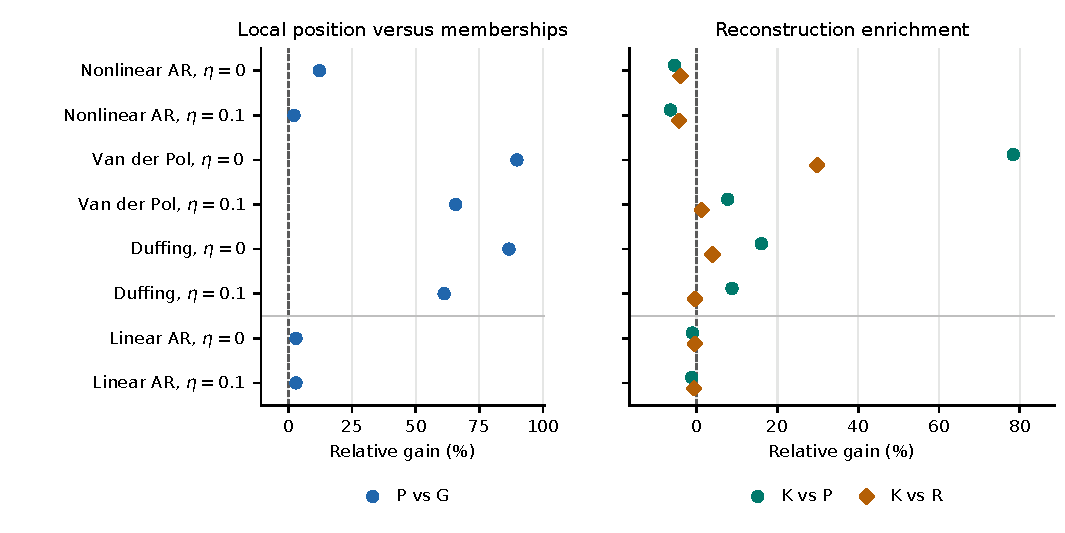
\includegraphics[width=\linewidth]{generated/soft_state_ablation/condition_gains.pdf}
\caption{Descriptive shared-bank gains by observation law and added
noise. Positive values favor the candidate. Each point uses all
\SARepetitions\ repetitions and averages the three horizons; the
condition displays have no separate confirmatory status. The complete
primary confidence family is in Table~\ref{tab:softstate-primary}.}
\label{fig:softstate-conditions}
\end{figure}

The Supplementary Studies reports all law/noise and horizon losses,
both cap-selection contexts, dimensions, and resource accounting.
Selected G, P, and K/R widths are $14$, $28$--$182$, and
$196$--$350$, respectively, for history width twelve. These descriptors
are therefore not a compression claim. Complete fitting and selection
uses \SAFitWallHours\ summed worker wall hours and
\SAFitCPUHours\ CPU hours; D prediction adds
\SAPredictionWallSeconds\ summed worker wall seconds.
Peak measured worker memory is \SAPeakWorkerRSSMiB\ MiB. These costs
include all candidates and reused geometry. Summed worker time is
not elapsed parallel runtime, and the measurements do not identify
isolated K versus R deployment costs. Preparation, audit and document
production are outside these fitting-and-prediction measurements.

Every planned task and primary contrast is retained. The source,
budget, menu and comparison family were unchanged after publication;
unfavorable comparisons did not trigger additional repetitions.
The experiment establishes finite direct-readout utility under the
specified laws and allocation. It does not test autonomous coordinate
propagation, Markov sufficiency, or a generally preferable forecasting
policy.

\section{Joint input-scaling and dimension selection}
\label{sec:joint-selection}

The preceding experiment selects local dimension while fixing input
standardization. Since input scaling changes distances, partitions,
principal directions, and projected kernels, dimension selection alone
does not exhaust the declared geometry choices. We therefore conducted
a separately frozen experiment in the same representation-only architecture.
It uses fresh repetitions and evaluates both enrichment of a common
geometry and the performance of individually selected procedures.
The completed preceding experiment remains unchanged; its terminal
observations are neither fitting or validation data for this study
nor pooled with this cohort. All 256 tasks and the independent
computational audit have completed.

\paragraph{Candidate geometry and unchanged decoder.}
Let $T_s$ denote an input transform fitted on the A histories and let
$c$ be a native local-dimension cap. The ordered grid is
\[
 \mathcal S\times\mathcal C
 =\{\text{standard},\text{min--max},\text{tanh}\}
   \times\{1,2,4,8,12\}.
\]
Standardization uses A population means and standard deviations.
Min--max uses A extrema, maps nonconstant A coordinates to $[-1,1]$,
and does not clip subsequent queries. An exactly constant A coordinate
is mapped to zero. The tanh transform is
$\tanh((x_k-\mu_{A,k})/\sigma_{A,k})$, with the inherited
small-scale rule and no subsequent input restandardization.
For every pair, one A-fitted bank supplies all four arms. The
partition sizes, reference limit, kernel construction, blockwise
standardization and radial maps, and ridge grid remain as in
Section~\ref{sec:softstate-study}. Thus G and P retain their exact
shared-prefix identities inside each candidate. Scaling can change
the bank across candidates; it is not assumed to preserve the same
geometry or numerical information.

For arm $a$, horizon $h$, scaler $s$, and cap $c$, B selects the ridge
penalty $\widehat\lambda_{a,h}(s,c)$ from the same five penalties.
The geometry score is
\begin{equation}
 Q_a(s,c)=\frac{1}{3}\sum_{h\in\{1,4,12\}}
 \frac{\MSE_{B,h}\!\left(\widehat f_{a,h,s,c,
       \widehat\lambda_{a,h}(s,c)}\right)}
 {\max\{\Var_A(Y_h),10^{-12}\}}.
 \label{eq:joint-selection-score}
\end{equation}
All coefficients, input transforms, and feature transforms are fitted
on A. Selected states are retained without a subsequent A+B refit.
C is diagnostic only and D is terminal evaluation only. Ties choose
the first scaler in the displayed order and then the first ascending
cap; penalty ties likewise choose the first grid entry.

\paragraph{Structural and complete-procedure comparisons.}
In the joint shared-bank view, P minimizes $Q_P(s,c)$ and all arms
use that bank with their own penalties. In the joint independent
view, each arm minimizes its own $Q_a(s,c)$. These views respectively
test enrichment of a selected common representation and the
performance of a complete tuned procedure. Neither compares a
K-selected geometry against a control arbitrarily held to P's bank.
Two standard-only views restrict the identical cached fits to
$s=\text{standard}$, selecting either with P or separately for each
arm. No additional models are fitted for these references. They
isolate the effect of expanding the scaling menu on the same fresh
cohort. Inclusion of the standard-only candidates guarantees a
weakly smaller selected B score for each arm in the independent
view and for P in the shared view. It gives no such guarantee for
the other arms on P's selected bank, or for any terminal loss.

\paragraph{Fixed cohort and primary comparisons.}
The experiment has 32 new independent repetitions and 256 task suites,
with the same laws, noise levels, histories, horizons, and A/B/C/D
allocation as the preceding study. A new master seed and an explicit
predecessor-stream exclusion check preceded generation. The protocol,
source, analysis, and independent audit were frozen and the source
published as commit \texttt{8e025027} before production preparation.
The fitted-state roster was sealed before D generation and the
terminal forecasts were sealed before target release and scoring.

One six-contrast primary family contains the four shared-bank
questions from the preceding study and two direct tests of joint
tuning: independently joint-selected K versus independently
dimension-selected standard-only K, with a 3\% nonlinear superiority
margin and a 5\% linear noninferiority margin. Repetition aggregates
remain the inferential units. The upper bound for a margin-adjusted
paired difference is
$\overline d+t_{1-0.05/6,31}s_d/\sqrt{32}$; a criterion is established
only when this bound is negative. Independent K/R comparisons and
law, noise, horizon, and selection-frequency breakdowns are
descriptive. The finite search does not globally optimize every
geometry parameter or establish autonomous soft-state dynamics.

\begin{table}[tbp]
\centering\small
\setlength{\tabcolsep}{4pt}
\begin{tabular}{@{}lllrrc@{}}
\toprule
Panel & Contrast & Criterion & Gain (\%) & $U$ & Met \\
\midrule
Nonlinear & $P/G$ & 3\% superiority & 68.69 & -0.0587852 & Yes \\
Nonlinear & $K/P$ & 3\% superiority & 8.86 & -0.00144862 & Yes \\
Nonlinear & $K/R$ & 3\% superiority & -0.9186 & 0.00119423 & No \\
Linear & $K/P$ & 5\% noninferiority & -1.26 & -0.0305374 & Yes \\
Nonlinear & $K_{\mathrm{joint}}/K_{\mathrm{standard}}$ & 3\% superiority & 0.0727 & 0.000901116 & No \\
Linear & $K_{\mathrm{joint}}/K_{\mathrm{standard}}$ & 5\% noninferiority & -0.2491 & -0.0417521 & Yes \\
\bottomrule
\end{tabular}

\caption{Six primary comparisons in the joint-selection experiment.
The first four use P's selected common bank; the last two compare
independently selected K procedures on the same cohort. Gain is
$100(1-\overline L_{\rm candidate}/\overline L_{\rm reference})$,
so a negative value means higher candidate loss. $U$ is the
simultaneous upper bound for the margin-adjusted paired difference;
the criterion is established only if $U<0$. Nonlinear criteria
require 3\% superiority and linear criteria allow 5\% noninferiority.}
\label{tab:joint-primary}
\end{table}

\paragraph{Shared geometry: useful enrichment without K/R superiority.}
Table~\ref{tab:joint-primary} establishes four of the six primary
criteria. In the shared-bank nonlinear population, P improves G
by \JSGainPG\% and K improves P by \JSGainKP\%; both simultaneous
bounds establish their 3\% margins. K's loss is
\JSRelativeLossChangeKR\% higher than R's, so the K/R superiority
criterion is not established. The corresponding nonlinear means
are \JSLossSharedNonlinearK\ for K and
\JSLossSharedNonlinearR\ for R. In the linear population, K's
loss is \JSRelativeLossChangeLinearKP\% higher than P's, while
the bound establishes the specified 5\% noninferiority margin.
Thus the position and conditional KAHM-enrichment findings persist
on fresh repetitions after expanding the geometry menu, but this
experiment supplies no KAHM-specific advantage over the matched RBF
construction.

\paragraph{Complete K procedure: little aggregate gain from the larger menu.}
Independently joint-selected K has nonlinear mean loss
\JSLossIndependentNonlinearK, versus
\JSLossStandardIndependentNonlinearK\ for independently
dimension-selected standard-only K. The point improvement is only
\JSGainJointKNonlinear\%, and the simultaneous bound does not
establish the prescribed 3\% superiority margin. On the linear
population, joint K's loss is
\JSRelativeLossChangeJointKLinear\% higher, while its bound
establishes 5\% noninferiority. The two direct tuning criteria
therefore do not jointly establish improved nonlinear performance
with linear noninferiority. This is a same-cohort comparison of selected
procedures; its small point difference is neither a guaranteed
benefit from extra choices nor evidence of equivalence.

\begin{figure}[tbp]
\centering
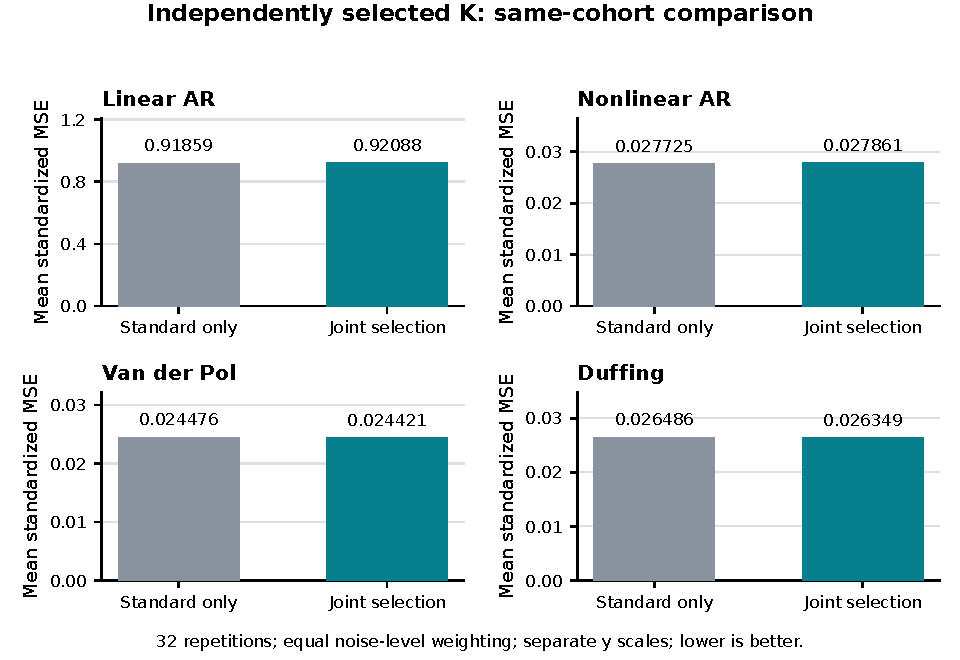
\includegraphics[width=0.88\linewidth]{generated/joint_selection/independent_K_joint_vs_standard.pdf}
\caption{Independently selected K with standard-only and joint
input-scaling menus. Each mean equally weights the two noise
conditions within each of 32 repetitions. All panels use a zero
origin but have separate vertical scales; lower loss is better.
The law-level comparisons are descriptive, with no uncertainty
intervals shown. Small oscillator gains accompany a nonlinear-AR
penalty, giving only a \JSGainJointKNonlinear\% aggregate nonlinear
gain under the prespecified weighting.}
\label{fig:joint-scaling}
\end{figure}

The law-level point comparisons in Figure~\ref{fig:joint-scaling}
show small gains for Van der Pol and Duffing and higher loss for
nonlinear autoregression. Joint K has lower nonlinear aggregate
loss in 15 of the 32 repetition pairs and higher loss in 17.
Independent K/R is also descriptive: K's nonlinear mean
\JSLossIndependentNonlinearK\ exceeds R's
\JSLossIndependentNonlinearR. These summaries do not replace
the six primary decisions. Selection frequencies, all four views,
resource records, and audit scope are retained in
the joint-selection section of the Supplementary Studies.
\FloatBarrier

\section{Context from preceding forecasting studies}
\label{sec:experiment}

The preceding studies evaluate complete forecasting procedures and
residual corrections. They provide context for the representation
ablation without supplying additional observations to its primary
analysis. Each retains its original cohort, selection rules, comparison
family, and numerical outcomes. Appendix~\ref{app:reconstruction-results}
gives the dimension-study protocol and complete results; the
\emph{Supplementary Studies} gives the later protocols and detailed tables.

\subsection{Validation-selected local dimension}

The earlier dimension experiment compares ten procedures on four laws
(nonlinear autoregression, Van der Pol, Duffing, and linear AR(2)), two
added-noise levels, and 24 independent repetitions: 192 tasks. Histories
have width twelve and horizons $1,4,12$. Independent episode sets
A/B/C/D contain 64/32/32/128 episodes: A fits scalers, banks and heads;
B selects hyperparameters; C calibrates corrections and selects the
non-KAHM procedure; D evaluates frozen forecasts. A/B/C retain at most
512/256/256 histories, and D uses all 1,664 origins. Source and analysis
were frozen locally before generation; predictions were sealed before
D-target release. This was not public preregistration.

Common, KAHM, and RBF procedures select their native cap independently
from $1,2,4,8,12,20$. Primary comparisons therefore need not share a bank;
secondary matched-bank comparisons hold the KAHM-selected bank fixed.
All non-ridge candidates are calibrated toward the same raw-ridge
baseline. The non-KAHM policy selects among ridge, raw RBF, boosting,
persistence, common features, and bounded or unbounded RBF departures.
Its comparison assesses a complete procedure, not matched feature capacity.
Native caps twelve and twenty coincide at the tested history width;
ascending ties select twelve. Native dimension permits full ambient rank.
The historical fixed-cap-two control retains its specified
$\min\{2,d-1,n_j-1\}$ restriction.

Task SMSE averages D mean squared errors divided by the corresponding
A-target variances across horizons. Nonlinear repetition loss averages
the three nonlinear laws and both noise levels; the linear panel is
separate. The five nonlinear margin contrasts are
$d_r=0.97L_{r,m}^{\mathrm{NL}}-L_{r,K}^{\mathrm{NL}}$;
the linear contrast is
$d_r=1.05L_{r,\mathrm{ridge}}^{\mathrm{lin}}-L_{r,K}^{\mathrm{lin}}$.
Each criterion requires
$\bar d-t_{23,1-0.05/6}s_d/\sqrt{24}>0$.
This is an approximate one-sided Bonferroni paired-$t$ calculation
across 24 independent repetition aggregates, not across dependent origins.
The declared joint criterion requires all six comparisons and the
separate numerical screens to pass.

\begin{table}[t]
\centering\small
\setlength{\tabcolsep}{3.5pt}
\caption{The preceding dimension study's unchanged six-claim family.
$L_K,L_m$ are mean SMSEs. Gain is $100(1-L_K/L_m)$.
The first five rows test a 3\% nonlinear improvement and the last a
5\% linear noninferiority tolerance. The simultaneous lower endpoint
concerns the absolute margin contrast; a positive endpoint establishes
the criterion. The complete ten-procedure results remain in the appendix.}
\label{tab:mechanism-primary}
\begin{tabular}{@{}lrrrrrc@{}}
\toprule
Comparator & $L_K$ & $L_m$ & Gain (\%) & $\bar d$ & Lower bound & Established \\
\midrule
Common features & 0.02891 & 0.03178 & 9.01 & 0.001910 & 0.001529 & Yes \\
Bounded RBF departure & 0.02891 & 0.02912 & 0.72 & -0.000663 & -0.000800 & No \\
Raw RBF & 0.02891 & 0.03143 & 8.01 & 0.001574 & 0.001156 & Yes \\
Boosted trees & 0.02891 & 0.02962 & 2.39 & -0.000181 & -0.000662 & No \\
Selected non-KAHM & 0.02891 & 0.02778 & -4.08 & -0.001967 & -0.002218 & No \\
Raw ridge (linear NI) & 0.90342 & 0.90166 & -0.20 & 0.043324 & 0.041880 & Yes \\
\bottomrule
\end{tabular}

\end{table}

KAHM's nonlinear loss is 0.028912. Its gains over common features and
raw RBF, \DFGainCommon\% and \DFGainRawRBF\%, establish their
3\% margins. Gains over independently selected RBF departures
(\DFGainRBF\%) and boosting (\DFGainHGB\%) do not; loss is
\DFWorsePolicy\% higher than the selected non-KAHM procedure.
Linear noninferiority passes: three of six criteria are established,
so the joint performance criterion fails. An unestablished margin does
not imply equality.

Dimension selection lowers loss relative to fixed cap two by
\DFDimensionGain\%, whereas native cap twenty raises it by 8.39\%.
On the KAHM-selected bank, the total loss change $-0.000973$ comprises
a common-feature improvement $-0.002150$ and a weakening of the
incremental departure benefit by $+0.001177$. This descriptive fitted-loss
decomposition is not a causal or orthogonal variance decomposition.
Matched-bank KAHM improves over RBF by 0.68\%, without establishing
the primary 3\% margin. All 192 tasks complete, the feature and
correction bounds have no violations, and the maximum taskwise
KAHM-to-ridge maximum-error ratio is \DFMaxErrorRatio{}, below five.
These checks establish computational coverage, not forecasting superiority.

\subsection{Preprocessing and residual-target follow-ups}
\label{sec:followup-experiments}

Both follow-ups use the same four laws, width-\PPHistory\ histories,
horizons $1,4,12$, and \PPTasks\ tasks per cohort. Preprocessing has
\PPRepetitions\ fresh repetition units. The residual-target results
are a same-cohort computational reproduction of the original
\CFRRepetitions\ units, with \CFRAdditionalRepetitions\ additional
independent repetitions. Each retains a separate four-claim family,
one-sided Bonferroni paired-$t$ bounds with 23 degrees of freedom,
3\% nonlinear superiority margins, and 5\% linear noninferiority.

\paragraph{Preprocessing.}
B jointly selects transformation and native cap. Candidate transforms
are standardization, unclipped min--max scaling, and $\tanh$ of
standardized histories; the five common/departure pairs include both
min--max/tanh hybrids. The selected KAHM procedure has
\PPRBFPenalty\% higher nonlinear loss than independently selected RBF
and \PPPolicyPenalty\% higher loss than the non-KAHM policy.
Tanh/tanh has \PPTanhPenalty\% higher loss than standard/standard.
Only linear noninferiority passes, despite observed excess loss
\PPLinearPenalty\%: \PPPrimaryEstablished\ of \PPPrimaryCount\ criteria.
A separate secondary design fits a common forecast on 32 episodes and
corrections on 32 disjoint episodes. Across its five scaler pairs,
KAHM reduces loss by \PPFixedBiasGainMin--\PPFixedBiasGainMax\% versus
the identical common-plus-bias baseline and
\PPFixedRBFGainMin--\PPFixedRBFGainMax\% versus independently selected
RBF. These descriptive gains do not reverse the primary result.

\paragraph{Residual targets.}
The next design retains a B-selected common forecast fitted on all
\CFREpisodesA\ A episodes and a shared B residual-mean bias $\beta_h$:
\begin{equation}
 \widehat f_{m,h}(x)=f_{\mathrm{base},h}(x)+\eta_{m,h}\delta_{m,h}(x),
 \qquad f_{\mathrm{base},h}=f_{\mathrm{com},h}+\beta_h,
 \quad\eta_{m,h}\in\{0,\tfrac14,\tfrac12,1\}.
 \label{eq:followup-fixed-common}
\end{equation}
The centered bounded departure slope $\delta_{m,h}$ adds no residual-mean
intercept. Four episode-wise folds produce out-of-fold (OOF) targets
from 48-episode common predictors; the in-sample alternative uses the
64-episode deployed common predictor. Both use full-A departure banks,
with independently B-selected scalers, caps and penalties and C-selected
multipliers. The comparison changes residual generation and resulting
selection, not just one target vector at fixed settings.

OOF KAHM improves the shared baseline by \CFRGainBias\%, establishing
its 3\% margin. The \CFRGainRBF\% gain over independently selected
OOF RBF does not establish that margin; loss is \CFRPolicyPenalty\%
higher than the expanded non-KAHM policy. Linear noninferiority passes
with observed excess \CFRLinearPenalty\%: \CFRPrimaryEstablished\ of
\CFRPrimaryCount\ criteria. The secondary in-sample correction has
SMSE \CFRISLoss{}, improving the shared baseline by \CFRISGainBias\%
and independent in-sample RBF by \CFRISGainRBF\%, yet remaining
\CFRISPolicyPenalty\% above the policy in a post hoc mean comparison.
OOF KAHM is \CFROOFvsISPenalty\% worse than in-sample KAHM, which is
lower in all \CFRRepetitions\ nonlinear repetition aggregates.
Different fold-training sizes and fitted settings limit causal attribution.

Original completed residual-study records were unavailable; the
reproduction uses the prescribed streams and unchanged scientific code
with prior outcome knowledge. Its audit verifies the newly retained
execution, including \CFRAuditArrays\ forecast arrays, without
authenticating the missing original records or creating a fresh
confirmatory cohort. Secondary comparisons retain their descriptive
status irrespective of their effect sizes.

\FloatBarrier
\subsection{Policy augmentation and a separate natural panel}
\label{sec:policy-augmentation}

A subsequent frozen policy study asks whether making the in-sample KAHM
correction available improves selection. It uses \PARepetitions\ fresh
repetitions and \PATasks\ tasks under the same laws and A/B/C/D roles;
earlier outcomes informed its design. $P_0$ selects one family from the
ten-family non-KAHM menu on C. $P_1$ adds the centered KAHM correction
in Equation~\eqref{eq:followup-fixed-common}; $P_0^+$ instead adds a
centered raw-history Nystr\"om RBF correction. Both additions retain the
same common forecast and shared bias and receive fifteen feature
configurations, five ridge penalties, and one added C-selection slot.
Equal search counts do not match width, statistical capacity, or runtime.
C calibrates each horizon and chooses a complete family; ties retain
the existing menu. A lower selected C loss need not imply lower D loss.

Nonlinear mean SMSEs are 0.02726839 for $P_0$, 0.02704583 for $P_1$,
and 0.02722502 for $P_0^+$. The gains \PAGainPZero\% and
\PAGainExtra\% fall below the prescribed 3\% margins. For
$d_r=L_{P_1,r}-aL_{Q,r}$, where $a=0.97$ for nonlinear superiority
and $a=1.05$ for linear noninferiority, the separate four-claim family
requires
\begin{equation}
 \bar d+t_{23,1-0.05/4}\,s_d/\sqrt{24}<0.
 \label{eq:pa-primary-bound}
\end{equation}
Both linear noninferiority criteria and neither nonlinear superiority
criterion are established (Table~\ref{tab:pa-primary}). This approximate
repetition-level paired-$t$ inference does not exclude a smaller benefit.

\begin{table}[t]
\centering\small
\caption{The preceding policy study's four original criteria, preserved
separately from the representation ablation. Gain is
$100(1-\overline L_{P_1}/\overline L_Q)$; the adjusted upper endpoint
concerns the absolute margin contrast in
Equation~\eqref{eq:pa-primary-bound}. A negative endpoint establishes
the criterion.}
\label{tab:pa-primary}
% Generated by build_policy_assets.py; do not edit.
\begin{tabular}{@{}llrrrl@{}}
\toprule
Panel & Comparator & Margin & Gain (\%) & Upper bound & Established \\
\midrule
Nonlinear & $P_0$ & 3\% & +0.8162 & +0.000711 & No \\
Nonlinear & $P_0^+$ & 3\% & +0.6582 & +0.000798 & No \\
Linear & $P_0$ & 5\% & -0.0016 & -0.044648 & Yes \\
Linear & $P_0^+$ & 5\% & +0.0016 & -0.044677 & Yes \\
\bottomrule
\end{tabular}

\end{table}

KAHM is selected in \PASyntheticSelections\ tasks: 43 nonlinear and
one linear. Among the nonlinear selections, thirty improve D loss and
thirteen worsen it; these conditional counts are descriptive. Standalone
KAHM improves the identical common-plus-bias baseline by
\PAMechanismBiasGain\% and independent local RBF by
\PAMechanismRBFGain\%, but has \PAStandalonePolicyPenalty\% higher
mean nonlinear loss than $P_0$. Useful residual correction therefore does
not establish the declared policy advantage.

\paragraph{Natural-series evaluation.}
A separate panel uses 24 Weekly and 24 Hourly M4 training series, chosen
by fixed ID hashes and length eligibility while excluding 72 earlier
pilot IDs \citep{M4DataSnapshot2026}. No official Test data are used.
Chronological A/B/C/D blocks have twelve intervening origins; D has
32 rolling origins at horizons $1,4,12$. Every target in one block is
observed before the next begins. Models remain fixed; later histories
may include earlier outcomes already observed at that origin. Seasonal
naive and drift replace the episode-OOF RBF family, giving eleven base
families and twelve per enlarged menu.

Overall SMSE is 0.127612 for $P_0$, 0.130512 for $P_1$, and 0.134159
for $P_0^+$. Augmentation is \PANaturalPenalty\% worse than the base
policy, despite being \PANaturalGainExtra\% better than the alternative
enlargement. Only \PANaturalSelections\ of \PANaturalSeries\ decisions
change: one improves and two worsen; the other 45 forecasts equal $P_0$.
Losses average horizons within series, series within frequency, and
frequencies equally; scales use A alone. Anonymous series may share
sources, so these results have no independence-based confidence interval.
They are descriptive benchmark-development evidence, not an official
M4 ranking or a new population-level superiority claim.

The audits cover 9,600 synthetic and 2,016 natural forecast arrays.
Synthetic source publication preceded terminal generation; the natural
protocol was frozen locally before parsing values and published after
evaluation. Neither is public preregistration. Complete grids, primary
bounds, selected cases, frequency losses, and audit limits remain in the
\emph{Supplementary Studies}. Any selector redesigned from these terminal
outcomes requires newly reserved evaluation.

\subsection{Earlier evidence and limits of transfer}
\label{sec:supporting-evidence}

The older investigations use their own geometric encodings, rank
policies, targets and inferential families; they are not interchangeable
instances of the present soft-state map. The \emph{Supplementary Studies}
retains their full methods, tables, proofs, and failure accounting.

Controlled target interventions show why reconstruction fidelity alone
can lose predictive position: an affine reconstruction can be nearly
exact while a discrepancy-based code discards the relevant coordinate.
Local position restores prediction in that example. Separate finite-decoder
comparisons favor KAHM on Van der Pol but favor controls on nonlinear
autoregression or Duffing. Thus their positive findings depend on the
law and decoder.

On four reserved natural source families, raw-history augmentation with
KAHM has 4.26\% higher source-balanced loss than raw RBF and costs
2.30 times as much; ridge is more accurate than both. Post hoc scaling
changes preserve the principal aggregate ordering. Additive corrections
yield some synthetic gains, but eight failed geometric fits and four
unavailable policy outputs prevent their planned complete archive
comparison. A post hoc successful-subset gain does not repair that
missing aggregate.

The learned-metric donor-residual study completes all 48 tasks and
improves on ridge, but its metric-versus-identity and donor-versus-in-sample
intervals include zero, and no adjusted comparison against an equally
trained geometric control favors KAHM. Direct reconstruction training
has two favorable, six unfavorable and ten unresolved primary contrasts;
neither favorable result is against an equally trained local control.
Three infeasible rideshare series leave its planned natural aggregate
undefined. Both online capacity settings fail their accuracy criteria,
and severe extrapolation persists after a solver correction. The present
bounded fixed-geometry decoder is a different procedure; its bound does
not retrospectively validate the adaptive method.

These outcomes constrain transfer beyond the specified constructions.
Their observations are not pooled with either the later forecasting
studies or the new representation ablation.

\section{Discussion and conclusion}\label{sec:discussion}

The four-arm comparison gives the soft-state viewpoint a specific
empirical question: which geometric observables help a fixed family of
readouts predict an external target? P versus G isolates access supplied
by local position; K versus P asks whether KAHM departures add useful
functions; K versus R asks whether that increment exceeds a matched
positive-kernel reconstruction. These are different claims. Success
for position does not establish a KAHM-specific advantage, and an
advantage over memberships alone does not establish sufficient state
representation.

The first experiment's complete primary family establishes three of
four criteria.
Position reduces nonlinear loss by \SAGainPG\% relative to
memberships, and KAHM departures reduce P's loss by \SAGainKP\%;
both exceed their $3\%$ margins under the simultaneous bounds.
The K/R gain is only \SAGainKR\%, so the KAHM-specific margin is
unestablished. K's linear loss is $1.11\%$ higher than P's, while
meeting the specified $5\%$ noninferiority criterion. Consequently,
the strongest supported claim concerns useful within-region position
and conditional reconstruction enrichment. It does not identify
inverse-Gram reconstruction as generally preferable to the matched
positive-kernel construction. Nor does a large P/G gain show that
memberships have no predictive content: it shows their limitations
for this affine readout and allocation.

In that experiment, the primary bank is selected for P, so the comparison concerns
enrichment of a validation-selected common representation. It does
not optimize the bank independently for G, K, or R. The secondary
independent-cap analysis asks a different question about complete
procedures. A discrepancy between contexts can identify sensitivity
to geometry selection; it cannot replace a failed primary criterion.
Likewise, failure to establish a margin is not evidence of equivalence.
The block transformations preserve shared coordinates, but fitted
access still depends on radial scaling, regularization, sample size,
and the affine readout. The comparison does not estimate all
information retained by an abstraction.

The first experiment's secondary results reinforce that distinction. Independently
selected K and R attain nonlinear mean losses
\SALossIndependentNonlinearK\ and \SALossIndependentNonlinearR\;
the K/R point difference changes sign without establishing either
equivalence or a new primary claim. K improves P on the oscillators
but worsens it on nonlinear autoregression, and its aggregate
advantage is concentrated at the longest tested horizon. The
selected enrichments have more coordinates than the original
history, so predictive utility here is not evidence of compression.
The recorded costs cover the full candidate search with shared
computations; they do not establish equal computation between K
and R or an isolated cost advantage for either.

The raw-span results explain why a change in reconstruction rule need
not create a new predictive function. Matched KAHM and RBF augmented
spans coincide under the stated symmetry conditions, while irregular
reference configurations can separate them. Equality concerns
jointly variable coefficients, including common coordinates.
It does not equate departures added to a frozen forecast, nor does
it survive arbitrary nonlinear transformations as a general rule.
Conversely, a distinct raw function need not align with the target
or be estimable. Equal nominal width and a common ridge architecture
therefore provide useful controls without proving equal effective
capacity, conditioning, or computational cost.

Local dimension acts on several parts of this construction at once:
position coordinates, projected kernels and reconstruction departures.
Input scaling also changes those quantities. The second experiment in
Section~\ref{sec:joint-selection} addresses their joint selection
using a common-bank structural view and an independently selected
complete-procedure view, each with a same-cohort standard-only
reference. Four of its six primary criteria are established.
The shared-bank P/G and K/P nonlinear gains remain substantial,
but K's nonlinear loss is \JSRelativeLossChangeKR\% higher than
R's. Independently expanding K's scaling menu improves its
nonlinear mean loss by only \JSGainJointKNonlinear\%, leaving
the prescribed 3\% gain unestablished. Its linear loss is
\JSRelativeLossChangeJointKLinear\% higher, within the established
5\% noninferiority criterion. These direct tuning comparisons use
the identical fresh cohort and dimension-selected standard-only
controls; they do not attribute between-experiment differences to
scaling. Neither the shared-bank nor independent-procedure view
supports a general KAHM-over-RBF claim. A failed superiority margin
also does not establish equivalence or prove that every scaling
choice is irrelevant.

The finite grid deliberately leaves other geometry parameters fixed.
Its result concerns three input transforms, five native caps, and
the declared ridge grid under this data allocation, rather than a
global optimum over all models or preprocessing choices.
The historical dimension decomposition finds stronger common prediction
and a smaller incremental departure benefit after selection.
Native full ambient rank is admissible, with caps twelve and twenty
coinciding at history width twelve; neither fact guarantees accuracy.
The preceding preprocessing and residual-target results likewise
discourage universal rules about tanh scaling or cross-fitting.
Cross-fitted common predictors use fewer episodes and may choose
different settings, so their comparison with an in-sample correction
does not identify the effect of residual fitting alone.

Representation-only readouts also delimit what the earlier residual
gains establish. A retained raw-history predictor can supply information
absent from its correction features. Within that architecture, a
correction helps when its alignment with the retained residual
outweighs its squared magnitude. Generic ridge arguments bound the
correction, not the common forecast or total error. Radial bounding
does not remove sensitivity at signed-normalization fallback
boundaries. These mathematical controls apply to matched alternatives
and establish neither forecasting superiority nor rollout stability.

The completed policy study illustrates a further distinction.
Its standalone KAHM correction improves the common-plus-bias baseline
by \PAMechanismBiasGain\% and local RBF by
\PAMechanismRBFGain\%, yet remains
\PAStandalonePolicyPenalty\% worse than the base policy.
Admitting it produces gains of \PAGainPZero\% and
\PAGainExtra\% against the base and enlarged-RBF policies,
establishing neither superiority margin. Equal search counts control
added selection opportunities without equating cost or capacity.
The natural panel changes only three of forty-eight decisions,
improving one and worsening two, with a \PANaturalPenalty\%
aggregate penalty against the base policy. Its potentially dependent
sources and limited frequency coverage support descriptive conclusions,
not an official M4 ranking or a population-level superiority claim.

Coordinate dynamics remain a separate requirement.
Proposition~\ref{prop:soft-state-closure} applies the standard
observable-space criterion for exact deterministic closure to the
raw-span comparison. It does not exhibit an invariant representation
for the experimental processes. Under stochastic transitions, a
linear conditional-mean evolution can coexist with irreducible
realized-successor variation; iteration requires appropriate Markov
and time-homogeneity assumptions. The companion certificates
\citep{KumarKargaran2026Limits} specify a fixed simplex map,
evaluation law and norm-bounded prediction class. They do not
automatically apply to signed enriched features or potentially
unbounded observation residuals.

A propagation investigation would therefore need to evaluate both
direct and propagated readouts against the same observed outputs,
alongside held-out successor errors and sensitivity to the horizon.
Predicting each candidate's own coordinates changes the target with
the representation. Nearly constant coordinates may be easy to
propagate while discarding useful distinctions; low coordinate error
or an inconclusive lower certificate alone cannot establish utility.
Such evidence is necessary for a claim about useful autonomous
soft-state dynamics, rather than for the narrower direct-readout
comparisons considered here.

Further selector design should depend on available incremental
opportunity. Saved forecasts can quantify that opportunity and losses
from missed or harmful selections exploratorily. Limited opportunity
would direct attention to the observables or target alignment;
substantial opportunity would motivate a better selector.
Any design informed by terminal outcomes requires newly reserved
evaluation. Fresh repetitions of familiar laws, historical adaptive
failures, and limited modern forecasting benchmarks constrain the
external scope of either conclusion.

Geometry-induced soft-state abstractions are therefore a useful
organizing framework when membership, position and reconstruction
are evaluated as distinct observables. The two experiments
support the predictive value of position and a conditional KAHM
departure increment, while leaving a general KAHM-specific advantage
over matched RBF unestablished. The joint-selection experiment
also finds very little aggregate nonlinear benefit from expanding
K's input-scaling menu beyond dimension-selected standardization.
The raw-span theory explains possible
functional distinctions without turning them into a guarantee of
utility. Useful autonomous dynamics and practical policy gains remain
separate empirical questions. The evidence supports a representation
research program with explicit external targets and matched controls,
rather than a general forecasting-superiority claim.

\section*{Reproducibility and research transparency}

\paragraph{Completed joint-selection study.}
The separate experiment under
\path{extensions/soft_state_joint_selection_20261102} has a frozen
protocol, source, analysis, and audit. Its standard-only mode
reproduces the published model bitwise on manufactured inputs.
The miniature staged audit passes 39,324 checks on eight artificial
tasks; the statistical preflight passes 42 checks on fabricated
losses. These readiness checks are distinct from the completed
scientific production results.

Scientific source commit \texttt{8e025027} was published before
production preparation. Its nineteen extension files and repository
root tree were verified at
12:50:03 UTC on 2 November 2026; the source-freeze SHA256 begins
\texttt{0c3737ae8d407198}. The actual public commit and its exact
file roster are recorded separately from the reviewed local
checkpoint in \path{PUBLICATION.json}. Global fitted-state and
forecast seals precede D generation and target release, respectively.
Target release completed at 13:08:30 UTC, analysis at 13:08:50,
and the independent audit at 13:14:09.

The audit passed \JSAuditChecks\ checks on all \JSTasks\ tasks
and independently confirmed all six primary decisions. It refitted
all 76,800 B penalty-path forecast arrays and replayed 4,096
selected C and 4,096 selected D arrays. Maximum absolute forecast
discrepancies were $1.13\times10^{-10}$, $2.42\times10^{-12}$,
and $6.28\times10^{-12}$, respectively. It verified the source
and stage chain, seed exclusions, complete task and data rosters,
A-fitted scaling, native dimensions, common-coordinate identities,
B selections, standard-only comparators, and exported statistics.
There were zero numerical solver recoveries. The audit retains
its declared tolerances and uses saved fitted geometry and physical
episodes; it does not independently refit partition k-means or
reintegrate the physical laws. These procedural controls are not
independent preregistration, oversight, cryptographic target
isolation, or external scientific replication.

Compact results and losslessly compressed large tables and audit
records are published separately from the frozen source. An indexed
numerical archive preserves all portable fitted states, candidate
paths, forecasts, and underlying data, with member and archive
checksums. Restoration verifies exact original bytes. Completed
result publication \texttt{06df3ed4} and the subsequent
manuscript edition have separate identities.

\paragraph{Preceding fixed-standardization representation study.}

The four-arm implementation and analysis specification are maintained
under \path{extensions/soft_state_ablation_20261102}.
The protocol requires source publication before production preparation,
a sealed A/B fitted-state roster before D generation, and sealed
terminal forecasts before scoring. The fixed budget, primary family
and secondary contexts are specified before production outcomes.
Artificial checks cover shared blocks, full and zero rank, cap aliases,
ridge paths, portable state, numerical recovery, and staged execution.
A separate artificial audit reconstructs eight miniature tasks, and
a deterministic 32-repetition loss fixture checks the statistical
design. These checks test implementation behavior, not forecasting
performance.

Scientific source commit \texttt{2b7d19b5} was published and its
twenty-five files verified at 09:20:24 UTC on 2 November 2026.
The source-freeze SHA256 begins \texttt{2745d10525a8fbc1}; the
complete digest is retained in \path{PUBLICATION.json}, and the source
list in \path{freeze.json}.
Preparation finished at 09:20:57, all fits were sealed at 09:28:00,
D preparation finished at 09:28:33, and predictions were sealed
at 09:34:57. Target release followed at 09:35:11 and analysis at
09:35:18. These are recorded procedural controls, not independent
preregistration, oversight or cryptographic target isolation.

The independent production audit passed \SAAuditChecks\ checks
covering all \SATasks\ tasks. It independently refitted all $25{,}600$
B penalty-path forecast arrays using Cholesky normal equations,
and replayed $2{,}048$ selected C and $2{,}048$ selected D arrays
from the portable fitted geometry. Maximum absolute prediction
differences were $1.20\times10^{-11}$, $2.43\times10^{-12}$ and
$5.59\times10^{-12}$ respectively. It reconstructed histories and
targets from saved base episodes and reserved streams, checked
native dimensions and exact shared-coordinate identities, and
independently recomputed the primary and descriptive statistics.
It did not independently refit partition k-means or reintegrate the
physical laws. All planned tasks completed, with zero solver
recoveries and zero query-denominator fallback calls. One singleton
local model used the declared rank-zero wrapper at all five caps.

Compact results and the audit summary are published with
\path{analysis/} and \path{verification/}; lossless compressed files
retain the largest tables and full audit receipt. Their restoration
script verifies hashes before writing. An indexed numerical archive
retains full fitted states, forecasts, data and candidate paths,
while the public source can regenerate them. The paper includes
the generated display assets and can compile without numerical
archives or refitting. The completed result publication is
\texttt{65ecf679}; it is separate from the frozen scientific
source and the subsequent manuscript edition.

Historical evidence retains separate records and inferential units.
The dimension-study audit checks 192 tasks, 18,816 local bases and
27 analysis tables under \path{extensions/dimension_forecasting}.
The preprocessing study and residual reproduction are under
\path{extensions/preprocessing_dimension} and
\path{extensions/crossfit_residual_reproduction_20261101}.
The reproduction restores a prescribed computation with prior outcome
knowledge; it neither recovers missing original run records nor adds
a fresh confirmatory cohort. Its zero-rank verification correction and
numerical recoveries have separate provenance.

The policy records remain under
\path{extensions/policy_augmentation_20261101} and
\path{extensions/policy_augmentation_natural_20261101}.
Scientific source \texttt{b1915813} and result publication
\texttt{b5941040} identify that completed study.
Its simulation audit checks 192 tasks and 9,600 terminal arrays;
the natural audit checks chronology, 2,016 arrays and 144 policy
choices. Those audits reuse inherited feature maps and do not
independently refit every unselected candidate. Their detailed
coverage and limits remain in the Supplementary Studies.

Displayed empirical values are generated from the corresponding
study tables with input and output hashes. Full principal proofs
and the earlier dimension protocol remain in the main appendices;
the Supplementary Studies preserves later protocols and older
investigations. Source and manuscript editions have separate
identities. A document build, checksum verification, forecast replay
and independent refitting are distinct checks; none constitutes
external scientific replication.


\bibliography{references}
\bibliographystyle{tmlr}
\appendix
\FloatBarrier
\section{Reconstruction algebra and bounded residual decoding}
\label{app:reconstruction-mechanism}

This appendix analyzes fixed reference maps and their use by a specified
decoder. It establishes normalized-kernel identities, conditions for equality
or inequality of feature spans, and a bound on fitted residual corrections.
None of these statements assumes a particular time-series distribution or
guarantees a forecasting improvement. Unless another subscript is displayed,
vector norms are Euclidean norms. The numerical examples can be evaluated
with \path{extensions/reconstruction_mechanism/algebra.py}; their reference
banks are constructed independently of forecasting outcomes.

\subsection{Normalized kernel identities}

Let $q_1,\ldots,q_M\in\R^d$ be reference histories, and let
$Q\in\R^{M\times d}$ contain their transposes as rows. Let
$P\in\R^{d\times r}$ have orthonormal columns, with $1\leq r\leq d$,
and let $W\in\R^{r\times r}$ be a symmetric positive-definite precision
matrix for the projected coordinates. For a column-vector query
$z\in\R^d$, define the Gaussian kernel vector $k(z)\in\R^M$ by
\[
 k_i(z)=\exp\!\left[-\frac{
 (P^\top(z-q_i))^\top W(P^\top(z-q_i))}{2r}\right],
 \qquad i=1,\ldots,M.
\]
Let $K\in\R^{M\times M}$ be the reference Gram matrix, with
$K_{ij}=k_i(q_j)$. For $\lambda>0$, set
$C=(K+\lambda I_M)^{-1}$, where $I_M$ is the $M\times M$ identity
matrix, and let $\mathbf1_M$ be the length-$M$ vector of ones.
The matrix $K$ is symmetric positive semidefinite, so $C$ exists and is
symmetric positive definite. The KAHM and matched positive-kernel
reconstructions are
\begin{equation}
 A_K(z)=\frac{Q^\top Ck(z)}{\mathbf1_M^\top Ck(z)},\qquad
 A_R(z)=\frac{Q^\top k(z)}{\mathbf1_M^\top k(z)}.
 \label{eq:mechanism-normalized-maps}
\end{equation}
The first expression is defined wherever its signed denominator is nonzero.
The second denominator is positive for every finite query. The two maps
share the references and projected Gaussian kernel. Multiplying $k(z)$
by a common positive scalar cancels in either ratio, which justifies
subtracting the largest log-kernel value before query evaluation.

\paragraph{Target-transfer identity.}
For a query satisfying $s(z)=\mathbf1_M^\top Ck(z)\ne0$, define the
normalized weight vector $\omega(z)=Ck(z)/s(z)$. Its entries sum to one.
For any reference target vector $y\in\R^M$,
\[
 \omega(z)^\top y=
 \frac{k(z)^\top(K+\lambda I_M)^{-1}y}
 {k(z)^\top(K+\lambda I_M)^{-1}\mathbf1_M}.
\]
Thus target transfer is the ratio of two dual kernel-ridge predictions
with regularization matrix $K+\lambda I_M$ and no additional intercept:
one fitted to $y$, and one fitted to the constant target $\mathbf1_M$.
For an affine scalar function $f(q)=q^\top b+c$, with
$b\in\R^d$ and $c\in\R$, let $f(Q)=Qb+c\mathbf1_M$ be its reference
values. Then
\[
 \omega(z)^\top f(Q)-f(z)=\{A_K(z)-z\}^\top b.
\]
\begin{proof}[Proof of Proposition~\ref{prop:mechanism-krr}]
The definition gives
$\mathbf1_M^\top\omega(z)=s(z)/s(z)=1$. Because $C=C^\top$,
$\omega(z)^\top y=k(z)^\top Cy/s(z)$ and
$s(z)=k(z)^\top C\mathbf1_M$, proving the ratio identity.
For the affine function,
\[
 \omega(z)^\top f(Q)
 =\omega(z)^\top Qb+c\omega(z)^\top\mathbf1_M
 =A_K(z)^\top b+c.
\]
Subtracting $z^\top b+c$ proves the final identity.
\end{proof}

This identifies direct target transfer as a normalized kernel-ridge
construction. The ratio generally differs from the unnormalized
kernel-ridge predictor because its denominator depends on the query.
Similarly, $A_K(z)^\top b$ is normalized kernel ridge applied to the
restricted reference target $Qb$. For any reconstruction $A$, the identity
$A(z)+\{z-A(z)\}=z$ also implies a linear dependence among the raw input,
reconstruction, and residual when all three are included as unrestricted
linear features. These identities constrain claims about the resulting
function class while allowing useful parameterizations for a restricted
or regularized decoder.

\subsection{When reconstruction departures have the same span}

Let $\mu\in\R^d$ be the reference center and define the affine
reconstruction $A_A(z)=\mu+PP^\top(z-\mu)$. Fix a common scalar locality
gate $g(z)$, and define column-vector departures
\[
 d_K(z)=g(z)\{A_K(z)-A_A(z)\},\qquad
 d_R(z)=g(z)\{A_R(z)-A_A(z)\}.
\]
A feature span means the set of scalar functions obtained by finite linear
combinations of its coordinate functions. Let $\mathcal S_0$ be the span
of the gate $g(z)$ and the coordinates of $g(z)P^\top(z-\mu)$.
It contains every coordinate of $g(z)A_A(z)$.

\paragraph{Equal augmented feature spans.}
Suppose $K\mathbf1_M=\kappa\mathbf1_M$ for a scalar $\kappa$ and
$C$ leaves the augmented reference-coordinate space
$\mathcal V=\operatorname{span}\{\mathbf1_M,Q_{:1},\ldots,Q_{:d}\}
\subseteq\R^M$ invariant. Here $Q_{:j}$ denotes column $j$ of $Q$.
Then there exist $B\in\R^{d\times d}$ and $c\in\R^d$ such that
\[
 C\mathbf1_M=a\mathbf1_M,\qquad
 CQ=QB+\mathbf1_M c^\top,\qquad a=(\kappa+\lambda)^{-1}>0.
\]
For these coefficients,
\[
 A_K=\frac{B^\top A_R+c}{a},\qquad
 d_K=\frac{B^\top}{a}d_R+
 \left(\frac{B^\top}{a}-I_d\right)gA_A+\frac{gc}{a}.
\]
The span obtained by adjoining the coordinates of $d_K$ to
$\mathcal S_0$ is the same as that obtained by adjoining the coordinates
of $d_R$.
\begin{proof}[Proof of Proposition~\ref{prop:mechanism-redundancy}]
The constant-row-sum assumption implies
$(K+\lambda I_M)\mathbf1_M=(\kappa+\lambda)\mathbf1_M$,
so $C\mathbf1_M=a\mathbf1_M$. Since $K$ is positive semidefinite,
$\kappa\geq0$ and hence $a>0$. Invariance of $\mathcal V$ means each
column of $CQ$ can be expressed using $Q$ and $\mathbf1_M$, which gives
$B$ and $c$. Using symmetry of $C$ in
Equation~\eqref{eq:mechanism-normalized-maps},
\[
 A_K(z)=
 \frac{(CQ)^\top k(z)}{(C\mathbf1_M)^\top k(z)}
 =\frac{B^\top Q^\top k(z)+c\mathbf1_M^\top k(z)}
 {a\mathbf1_M^\top k(z)}
 =\frac{B^\top A_R(z)+c}{a}.
\]
Subtract $A_A$ and multiply by $g$ to obtain the displayed departure
identity. Since $gA_A=g\mu+P\{gP^\top(z-\mu)\}$, all its coordinates
belong to $\mathcal S_0$. Thus the KAHM-augmented span is contained in
the RBF-augmented span.

For the reverse inclusion, the restriction of the invertible matrix $C$
to the invariant finite-dimensional space $\mathcal V$ is injective and
therefore surjective onto $\mathcal V$. Its images
$C\mathbf1_M=a\mathbf1_M$ and the columns of $CQ$ consequently span
$\mathcal V$. Hence there exist $D\in\R^{d\times d}$ and $e\in\R^d$ such that
$Q=(CQ)D+\mathbf1_M e^\top$. Multiplying its transpose by
$k(z)/(\mathbf1_M^\top k(z))$ gives
$A_R(z)=aD^\top A_K(z)+e$. After multiplication by $g$ and subtraction
of $gA_A$, this expresses each RBF departure coordinate using KAHM
departure coordinates and $\mathcal S_0$. The spans therefore agree,
including when the original reference-coordinate columns are redundant.
\end{proof}

For example, take scalar references $q=(-1,1)^\top$, $P=1$, $g=1$,
and $A_A(z)=z$. If the off-diagonal Gram entry is $\rho$, then
$K\mathbf1_2=(1+\rho)\mathbf1_2$ and $Kq=(1-\rho)q$. Therefore
\begin{equation}
 A_K=c_\rho A_R,\qquad
 d_K=c_\rho d_R+(c_\rho-1)z,\qquad
 c_\rho=\frac{1+\rho+\lambda}{1-\rho+\lambda}.
 \label{eq:mechanism-two-reference}
\end{equation}
The coefficient $c_\rho$ is positive, so
$\operatorname{span}(1,z,d_K)=\operatorname{span}(1,z,d_R)$.
With the sample-variance precision $1/2$, $\rho=e^{-1}$.
The regularization iteration used by the implementation yields
$\lambda=2.6519665429866075$ and $c_\rho=1.224037566462905$.
The maximum numerical identity error on the constructed query grid is
below $6\times10^{-16}$.

These are equalities between untransformed feature spans. An isotropic
ridge penalty is not invariant under a general nonorthogonal change of
coordinates. Applying separate nonlinear radial transformations can also
remove the displayed linear relation. A forecasting comparison therefore
evaluates the complete reconstruction, feature transformation, and fitting
procedure, even when two untransformed feature sets have the same span.

\subsection{Freezing the common predictor}
\label{app:mechanism-fixed-common}

Consider the two-reference example in
Equation~\eqref{eq:mechanism-two-reference} on $\R$. For a Gaussian
kernel of positive precision, $0<\rho<1$, so $c_\rho>1$.
Writing $t>0$ for the scalar precision gives $A_R(z)=\tanh(tz)$,
which is bounded and nonconstant.
If $az+bd_R(z)=0$, then $(a-b)z+bA_R(z)=0$. Boundedness first gives
$a=b$, and nonconstancy then gives $b=0$. Thus $z$ and $d_R$ are
linearly independent. Were $d_K=u d_R$ for a scalar $u$,
Equation~\eqref{eq:mechanism-two-reference} would give
$(c_\rho-1)z+(c_\rho-u)d_R=0$, contradicting that independence.
The nonzero one-dimensional spans of $d_K$ and $d_R$ are therefore
distinct and neither contains the other. Translating both by any fixed
$f_{\mathrm{base}}$ proves the claims about
Equation~\eqref{eq:mechanism-fixed-common-classes}. Permitting the
coefficient of $z$ to vary restores the equal augmented spans already
proved above.

For a fixed fitting sample, define $H_Av(z)=v(z)-\bar v_A$. Linearity
gives
\[
 H_A d_K=c_\rho H_A d_R+(c_\rho-1)H_A z.
\]
The same non-equality argument applies whenever $H_Az$ and $H_Ad_R$
are linearly independent on the query domain under consideration.
On the whole real line this follows from independence of $1,z,d_R$:
boundedness and nonconstancy of $A_R$ prove it by the preceding argument
with an added constant. Independence need not hold on an arbitrary
finite query set. Separate nonlinear radial maps need not preserve
the displayed identity. These are function-class statements; they
give no risk ordering for fitted or calibrated forecasts.

\subsection{An explicit distinct reconstruction basis}

\paragraph{Irregular scalar references.}
Let $q_1<q_2<q_3$ with $q_1+q_3\ne2q_2$, and define
$k_i(z)=\exp\{-t(z-q_i)^2/2\}$ for precision $t>0$.
Let $K_{ij}=\exp\{-t(q_i-q_j)^2/2\}$,
$C=(K+\lambda I_3)^{-1}$ for $\lambda>0$, and suppose every entry of
$v=C\mathbf1_3$ is positive. For the reconstructions in
Equation~\eqref{eq:mechanism-normalized-maps}, with $Q=q=(q_1,q_2,q_3)^\top$,
gate $g=1$, and $A_A(z)=z$,
\[
 A_K\notin\operatorname{span}(1,z,A_R),\qquad
 d_K\notin\operatorname{span}(1,z,d_R).
\]
These are statements about scalar functions on the whole real line.
\begin{proof}[Proof of Proposition~\ref{prop:mechanism-distinct}]
Set $u=Cq$. Since $C$ is symmetric,
$A_K(z)=(k(z)^\top u)/(k(z)^\top v)$, and positivity of $v$ makes
its denominator positive for every $z$. The six sums $q_i+q_j$ with
$i\leq j$ are distinct: strict ordering of the three references orders
all the sums except possibly $q_1+q_3$ and $2q_2$, and their equality
is excluded by assumption. Products of Gaussian translates satisfy
\[
 k_i(z)k_j(z)=
 e^{-tz^2}e^{-t(q_i^2+q_j^2)/2}e^{t(q_i+q_j)z}.
\]
After removal of the common positive factor $e^{-tz^2}$, these products
are nonzero multiples of exponentials with six distinct real exponents.
Such exponentials are linearly independent. Indeed, differentiating a
vanishing linear combination zero through fifth order at $z=0$ gives
a Vandermonde system whose determinant is the product of the nonzero
pairwise exponent differences.

Suppose first that $A_K=cA_R+d$ for scalars $c,d$. Define
$w=u-dv$. Multiplication by the two positive denominators gives
\[
 \left(\sum_i k_iw_i\right)\left(\sum_j k_j\right)
 =c\left(\sum_i k_iq_i\right)\left(\sum_j k_jv_j\right).
\]
Independence of the six products implies equality of their coefficients.
The diagonal coefficients give $w_i=cq_iv_i$, and the off-diagonal
coefficients give
$w_i+w_j=c(q_iv_j+q_jv_i)$ for $i<j$.
If $c=0$, all $w_i$ vanish, so $Cq=dC\mathbf1_3$. Invertibility of
$C$ would imply $q=d\mathbf1_3$, contrary to the distinct references.
If $c\ne0$, substituting the diagonal equations into the off-diagonal
ones yields $(q_i-q_j)(v_i-v_j)=0$. Thus $v=a\mathbf1_3$ for some
$a>0$, and $(K+\lambda I_3)v=\mathbf1_3$ implies that $K$ has
constant row sums. This is impossible: its middle-row sum exceeds the
first-row sum by $K_{23}-K_{13}>0$ and the last-row sum by
$K_{12}-K_{13}>0$, since the Gaussian decreases strictly with positive
distance. This rules out every affine relation $A_K=cA_R+d$.

Both reconstructions are bounded functions of $z$. The RBF reconstruction
is a convex combination of $q_1,q_2,q_3$. Also,
\[
 A_K(z)=\frac{\sum_i k_i(z)v_i\,(u_i/v_i)}
 {\sum_i k_i(z)v_i}
\]
is a convex combination of the three finite numbers $u_i/v_i$.
If $A_K(z)=cA_R(z)+d+bz$ held on the real line, boundedness of both
reconstructions would force $b=0$. The affine relation already ruled out
would then follow. This proves the first span statement. Finally,
$d_K=A_K-z$ and $d_R=A_R-z$ imply
$\operatorname{span}(1,z,d_R)=\operatorname{span}(1,z,A_R)$.
Membership of $d_K$ in this span would imply membership of $A_K$, a
contradiction.
\end{proof}

A concrete example uses $q=(-1,0,2)^\top$, sample-variance precision
$t=3/7$, and $\lambda=4.498274743339644$ from the specified
regularization iteration. Positivity of $C\mathbf1_3$ can be verified
without examining a query grid. Write $K=I_3+E$ and $a=1+\lambda$.
For a matrix, let $\|\cdot\|_\infty$ denote the maximum absolute row
sum; for a vector, it denotes the largest absolute entry. If
$a>2\|E\|_\infty$, then the Neumann series for
$aC=(I_3+E/a)^{-1}$ gives
\[
 \|aC\mathbf1_3-\mathbf1_3\|_\infty
 \leq\sum_{j=1}^{\infty}(\|E\|_\infty/a)^j
 =\frac{\|E\|_\infty/a}{1-\|E\|_\infty/a}<1.
\]
Every entry of $aC\mathbf1_3$ is then strictly positive. In the example,
$\|E\|_\infty=e^{-3/14}+e^{-6/7}=1.2314905926823394$, so the
condition holds. On $81$ constructed queries in $[-3,4]$, the maximum
absolute residual after least-squares projection of the sampled $d_K$
values onto the sampled $(1,z,d_R)$ columns is
$0.05355670997078987$. This numerical illustration supplements the
analytic existence result. It does not establish distinctness for every
higher-dimensional bank used in the forecasting experiments.

\subsection{A bounded correction with a free intercept}

For a feature block $v\in\R^{p_b}$ of positive width $p_b$, define
\begin{equation}
 T_{R_b}(v)=\frac{v}{\sqrt{1+\|v\|_2^2/R_b^2}},\qquad
 R_b=\sqrt{p_b}.
 \label{eq:mechanism-radial}
\end{equation}
Its norm is at most $R_b$. To see its sensitivity to its own input, set
$a=1+\|v\|_2^2/R_b^2$. Its Jacobian is
$a^{-1/2}I-a^{-3/2}vv^\top/R_b^2$. For $v\ne0$, the eigenvalue in
the direction of $v$ is $a^{-3/2}$, and each orthogonal direction has
eigenvalue $a^{-1/2}$; at zero, the Jacobian is the identity. All its
singular values are therefore at most one. Integrating the derivative
along the segment between any two inputs proves
$\|T_{R_b}(v)-T_{R_b}(v')\|_2\leq\|v-v'\|_2$.
Thus the radial transformation is nonexpansive.

Concatenating separately transformed blocks gives a feature vector
$\psi(z)\in\R^p$, where $p=\sum_b p_b$, satisfying
$\|\psi(z)\|_2\leq R=(\sum_bR_b^2)^{1/2}$. This norm bound holds
wherever the preceding feature construction is defined. Nonexpansiveness
of the radial transformation does not by itself give a Lipschitz constant
for the full history-to-feature map, which includes the signed
reconstruction denominator and its fallback rule.

\paragraph{Centered ridge correction.}
For $n\geq1$, let $e_i\in\R$ be residual targets and
$\psi_i\in\R^p$ be training feature vectors. Fit $b\in\R$ and
$w\in\R^p$ by minimizing
\[
 \frac1n\sum_{i=1}^n(e_i-b-\psi_i^\top w)^2+\alpha\|w\|_2^2,
 \qquad\alpha>0,
\]
with no penalty on $b$. Define the training means
$\bar e=n^{-1}\sum_i e_i$ and
$\bar\psi=n^{-1}\sum_i\psi_i$, the residual vector
$e=(e_1,\ldots,e_n)^\top$, its centered version
$e_c=e-\bar e\mathbf1_n$, and its centered root mean square
$\sigma_e=\|e_c\|_2/\sqrt n$. Suppose query features satisfy
$\|\psi(z)\|_2\leq R$. Then, for any scalar $\gamma$,
\begin{equation}
 \|w\|_2\leq\frac{\sigma_e}{2\sqrt\alpha},\qquad
 |\gamma q(z)|\leq|\gamma|\left[
 |\bar e|+(R+\|\bar\psi\|_2)\frac{\sigma_e}{2\sqrt\alpha}\right],
 \quad q(z)=\bar e+(\psi(z)-\bar\psi)^\top w.
 \label{eq:mechanism-correction-bound}
\end{equation}
\begin{proof}[Proof of Proposition~\ref{prop:mechanism-correction-bound}]
For fixed $w$, differentiating with respect to the intercept gives
$b=\bar e-\bar\psi^\top w$. Let $\Psi_c\in\R^{n\times p}$ have
row $i$ equal to $(\psi_i-\bar\psi)^\top$. Substituting the fitted
intercept reduces the objective to
$n^{-1}\|e_c-\Psi_cw\|_2^2+\alpha\|w\|_2^2$.
Its unique minimizer is
\[
 w=(\Psi_c^\top\Psi_c+n\alpha I_p)^{-1}\Psi_c^\top e_c.
\]
For a singular value $s\geq0$ of $\Psi_c$, the corresponding singular
value of the coefficient operator is $s/(s^2+n\alpha)$. The inequality
$(s-\sqrt{n\alpha})^2\geq0$ implies
\[
 \frac{s}{s^2+n\alpha}\leq\frac{1}{2\sqrt{n\alpha}}.
\]
The operator norm is therefore at most $1/(2\sqrt{n\alpha})$, giving
$\|w\|_2\leq\|e_c\|_2/(2\sqrt{n\alpha})
=\sigma_e/(2\sqrt\alpha)$. Finally, the fitted intercept gives
$q(z)=\bar e+(\psi(z)-\bar\psi)^\top w$.
Cauchy--Schwarz and the triangle inequality yield
\[
 |q(z)|\leq|\bar e|+
 (\|\psi(z)\|_2+\|\bar\psi\|_2)\|w\|_2
 \leq|\bar e|+(R+\|\bar\psi\|_2)
 \frac{\sigma_e}{2\sqrt\alpha}.
\]
Multiplication by $|\gamma|$ proves the correction bound.
\end{proof}

The mean-squared-error objective corresponds to a summed-squared-error
objective with penalty $n\alpha$. Keeping the numerical value $\alpha$
unchanged when switching to a summed loss would define a different
estimator. For multiple forecast horizons, the bound applies separately
to each fitted residual vector and each selected pair
$(\alpha_h,\gamma_h)$. This is a general property of ridge regression
on bounded features, including the KAHM features considered here. It
bounds the additive correction but does not bound the retained raw
baseline or total forecast error. The experiment checks the feature,
coefficient, and correction inequalities on every saved task and reports
forecast errors separately.

\paragraph{Centered slope-only specialization.}
For Equation~\eqref{eq:mechanism-centered-slope-fit}, let $\Phi_c$
have rows $(\varphi_m(x_i)-\bar\varphi_m)^\top$ and let
$r_c=(r_{ih}-\bar r_h)_{i=1}^{n_A}$. Then
\[
 v_{m,h}=(\Phi_c^\top\Phi_c+n_A\alpha_{m,h}I)^{-1}\Phi_c^\top r_c.
\]
The same singular-value inequality gives the coefficient bound in
Equation~\eqref{eq:mechanism-centered-slope-bound}.
Cauchy--Schwarz applied directly to
$(\varphi_m(x)-\bar\varphi_m)^\top v_{m,h}$ gives its correction
bound, without a response-mean term. No intercept is reintroduced in
this deployed slope. Finally, writing
$e=Y-f_{\mathrm{base}}(X)$ gives
$(e-\eta\delta(X))^2-e^2=\eta^2\delta(X)^2-2\eta e\delta(X)$.
Finite second moments make all terms integrable and justify taking the
conditional expectation stated in
Equation~\eqref{eq:mechanism-residual-risk}. This identity uses no
independence assumption between the residual and the correction.

\FloatBarrier
\section{Earlier residual forecasting readouts}\label{app:earlier-decoders}

The completed residual-forecast studies read out future observations
through bounded features and retained baselines. This appendix preserves
their transformations, fitting rules, and generic ridge bounds.
Section~\ref{sec:bounded-decoder} specifies the direct affine readouts
for the G/P/K/R representation comparison, which separately transform
membership and position blocks. Neither architecture estimates or
iterates a transition matrix. Bounded decoder inputs are distinguished
from the raw observable spaces analyzed in
Section~\ref{sec:reconstruction-theory}.

\subsection{Joint common block and separate departure block}


Each feature block is centered and scaled coordinatewise using A alone;
feature standard deviations are floored at $10^{-6}$. A tilde denotes
this coordinatewise standardization. Apply the radial map
$T_R$ in Equation~\eqref{eq:mechanism-main-radial}, with $R=\sqrt p$
for a block of width $p$.
This radial map has norm at most $R$ and is nonexpansive with respect to
its argument. If the common and departure block dimensions are $p_0$
and $p_d$, respectively, set $R_0=\sqrt{p_0}$ and $R_d=\sqrt{p_d}$.
The bounded feature vectors are
\[
 \chi_K(z)=\operatorname{concat}\bigl(
       T_{R_0}(\widetilde\psi_0(z)),T_{R_d}(\widetilde d_K(z))\bigr),
 \qquad
 \chi_R(z)=\operatorname{concat}\bigl(
       T_{R_0}(\widetilde\psi_0(z)),T_{R_d}(\widetilde d_R(z))\bigr).
\]
The two blocks are transformed separately and are not standardized again.
Consequently, appending a departure does not rescale the common features.
For $J$ local models with stored ranks $r_j$, the dimensions are
$p_0=J+\sum_j r_j$ and $p_d=Jd$. The earlier dimension experiment requests
partitions with 2, 4, and 8 models and at most 24 references per model.
All fitted banks contain $J=14$ models, so $p_d=168$ for its
12-dimensional histories, whereas $p_0$ varies with the local ranks.
Each candidate geometry is fitted without targets on A and remains fixed
during selection and evaluation. All bounds use its actual dimensions.

\subsection{Fitting and calibrating the correction}

In the dimension study, let $f_{0,h}$ be the raw-history ridge baseline
for horizon $h$. Given
an unstandardized history $x$, let $\psi(x)$ denote a generic chosen
bounded feature vector, such as $\chi_K$ or $\chi_R$, after applying its
A-fitted input scaler. The forecast is
\begin{equation}
 \widehat y_{t+h}=f_{0,h}(x_t)+\gamma_h q_h(x_t),\qquad
 q_h(x)=b_h+\psi(x)^\top w_h.
 \label{eq:mechanism-main-forecast}
\end{equation}
Here $b_h\in\R$ is a free intercept, $w_h$ is the coefficient vector,
and $\gamma_h$ controls the correction strength. For $n_A$ fitting
histories, the residual targets are
$e_{ih}=y_{i,h}-f_{0,h}(x_i)$, where $y_{i,h}$ is the observed future
at horizon $h$ for fitting history $i$. The correction minimizes
\[
 \frac1{n_A}\sum_{i=1}^{n_A}
       \{e_{ih}-b_h-\psi(x_i)^\top w_h\}^2
       +\alpha_h\|w_h\|_2^2.
\]
When $\psi$ contains both common and departure blocks, their coefficients
are fitted jointly. Sharing the raw-history baseline and the common
feature construction therefore does not fix the fitted common
contribution across departure methods.
Set B selects $\alpha_h\in\{10^{-4},10^{-3},10^{-2},10^{-1},1\}$
by forecast error separately for each horizon and candidate cap.
For each geometric procedure $m$, let $\widehat y^{(c)}_{m,h}$ be its
B prediction after this penalty selection, with $\gamma_h=1$. One cap
is selected across horizons by
\begin{equation}
 \widehat c_m=\mathop{\arg\min}_{c\in\{1,2,4,8,12,20\}}
 \frac1{|\mathcal H|}\sum_{h\in\mathcal H}
 \frac{\MSE_B(Y_h,\widehat y^{(c)}_{m,h})}
 {\max\{\Var_A(Y_h),10^{-12}\}}.
 \label{eq:dimension-cap-selection}
\end{equation}
Here $\Var_A$ is the empirical variance of the retained A targets with
divisor $n_A$; exact ties select the smallest cap. The common, bounded
KAHM, bounded RBF, and two unbounded-departure procedures each make
their own choice. These choices are fixed before accessing C.
Set C then selects $\gamma_h\in\{0,1/4,1/2,1\}$ separately by
horizon. Neither selection step refits the geometry or decoder, and
set D is reserved for final evaluation. The cap objective uses
uncalibrated B forecasts, so C does not enter dimension selection.

\subsection{A uniform bound including the intercept}

Define the fitting residual mean, centered root mean square, and feature
mean as
\[
 \bar e_h=\frac1{n_A}\sum_i e_{ih},\qquad
 \sigma_{e,h}=\left[\frac1{n_A}\sum_i(e_{ih}-\bar e_h)^2\right]^{1/2},
 \qquad
 \bar\psi=\frac1{n_A}\sum_i\psi(x_i).
\]
\begin{proposition}[Centered ridge correction bound]
\label{prop:mechanism-correction-bound}
For the mean-squared-error objective above with $n_A\geq1$,
$\alpha_h>0$, and an unpenalized intercept, suppose that the feature
map satisfies $\|\psi(x)\|_2\leq R$ on its input domain.
For any scalar $\gamma_h$, the fitted coefficients and correction satisfy
\begin{equation}
 \|w_h\|_2\le\frac{\sigma_{e,h}}{2\sqrt{\alpha_h}},\qquad
 |\gamma_h q_h(x)|\le |\gamma_h|\left[
 |\bar e_h|+(R+\|\bar\psi\|_2)
 \frac{\sigma_{e,h}}{2\sqrt{\alpha_h}}\right].
 \label{eq:mechanism-main-correction-bound}
\end{equation}
\end{proposition}
For a concatenated bounded common and departure vector,
$R=\sqrt{R_0^2+R_d^2}$; for the common-only vector, $R=R_0$.
For this decoder, the free intercept contributes the residual-mean term
and cannot be omitted. This bound controls the correction, not the baseline, total
forecast error, or sensitivity of the preceding reconstruction to changes
in the history.


\paragraph{Proof idea.}
Eliminating the intercept gives
$b_h=\bar e_h-\bar\psi^\top w_h$. If $\Psi_c$ is the matrix whose
rows are $(\psi(x_i)-\bar\psi)^\top$ and $e_c$ is the centered
residual vector, then
$w_h=(\Psi_c^\top\Psi_c+n_A\alpha_h I)^{-1}\Psi_c^\top e_c$.
The coefficient operator has singular values
$s/(s^2+n_A\alpha_h)\leq1/(2\sqrt{n_A\alpha_h})$.
This yields the coefficient bound. Applying Cauchy--Schwarz to
$q_h(x)=\bar e_h+(\psi(x)-\bar\psi)^\top w_h$ yields the
correction bound. Appendix~\ref{app:reconstruction-mechanism} gives
the complete argument, including the nonexpansiveness of the radial map.

The proposition applies separately to each selected horizon and is a property
of bounded-feature ridge regression. A summed-squared-error objective
would need penalty $n_A\alpha_h$ to define the same estimator. The
radial transformation is nonexpansive in its own input, but this does
not give a Lipschitz bound for the preceding signed reconstruction or
for its fallback boundary.

\paragraph{Baseline recovery and predictive gain.}
The calibration grid includes $\gamma_h=0$, which recovers the same
fitted baseline exactly. This is an available forecast rather than a
guarantee that a finite calibration set selects the best future forecast.
The coefficient and correction bounds likewise make no claim about
prediction accuracy. The experiment therefore evaluates error, numerical
coverage, and the correction inequalities as separate outcomes.

\subsection{Centered corrections to a frozen common predictor}
\label{sec:fixed-common-decoder}

The residual-target study fixes a separately fitted common forecast
$f_{\mathrm{com},h}$ and a shared bias before comparing departures:
\begin{equation}
 f_{\mathrm{base},h}(x)=f_{\mathrm{com},h}(x)+\beta_h,\qquad
 \beta_h=\frac1{n_B}\sum_{i\in B}
       \{y_{i,h}-f_{\mathrm{com},h}(x_i)\}.
 \label{eq:mechanism-fixed-common-baseline}
\end{equation}
The common forecast is fitted on all of A and selected on B. Its
coefficients and the B-fitted bias are then shared across the departure
comparisons and frozen before C. Thus the common component cannot
compensate for a change of departure coordinates during residual fitting.

Let $\varphi_m(x)$ be the separately standardized and radially bounded
departure block for method $m$, with $\|\varphi_m(x)\|_2\leq R_{d,m}$,
and let $\bar\varphi_m$ be its A mean. For either in-sample or
out-of-fold residual targets $r_{ih}$, write
$\bar r_h=n_A^{-1}\sum_i r_{ih}$ and fit
\begin{equation}
 v_{m,h}=\mathop{\arg\min}_{v}\left[
 \frac1{n_A}\sum_i
 \{r_{ih}-\bar r_h-(\varphi_m(x_i)-\bar\varphi_m)^\top v\}^2
 +\alpha_{m,h}\|v\|_2^2\right],\qquad \alpha_{m,h}>0.
 \label{eq:mechanism-centered-slope-fit}
\end{equation}
In-sample targets use $r_{ih}=y_{i,h}-f_{\mathrm{com},h}(x_i)$;
out-of-fold targets use the common forecast fitted without the fold
containing the episode of $x_i$. The deployed forecast is
\begin{equation}
 \widehat f_{m,h}(x)=f_{\mathrm{base},h}(x)+\eta_{m,h}\delta_{m,h}(x),
 \qquad
 \delta_{m,h}(x)=(\varphi_m(x)-\bar\varphi_m)^\top v_{m,h}.
 \label{eq:mechanism-centered-slope-forecast}
\end{equation}
It contains no additional residual-mean intercept. Subtracting the
constant shared bias before centering the fitting targets would leave
the slope unchanged. The correction has zero empirical mean on A;
its mean on another distribution need not vanish. Setting $\eta_{m,h}=0$
recovers the same shared baseline for every departure method.

\paragraph{Bound for the deployed slope.}
Define $\sigma_{r,h}^2=n_A^{-1}\sum_i(r_{ih}-\bar r_h)^2$.
The spectral argument of
Proposition~\ref{prop:mechanism-correction-bound} immediately gives
\begin{equation}
 \|v_{m,h}\|_2\leq\frac{\sigma_{r,h}}{2\sqrt{\alpha_{m,h}}},\qquad
 |\eta_{m,h}\delta_{m,h}(x)|\leq
 |\eta_{m,h}|(R_{d,m}+\|\bar\varphi_m\|_2)
 \frac{\sigma_{r,h}}{2\sqrt{\alpha_{m,h}}}.
 \label{eq:mechanism-centered-slope-bound}
\end{equation}
The residual-mean term is absent because it is absent from the deployed
correction. The fixed common forecast and shared bias remain outside
this bound. This specialization is generic bounded-feature ridge
algebra and applies equally to the matched RBF departure.

\paragraph{Residual alignment and predictive gain.}
Condition on all fitted and selected quantities, and take expectations
under a specified evaluation distribution for $(X,Y)$. Suppress the
horizon and method indices, and suppose $Y$, $f_{\mathrm{base}}(X)$,
and $\delta(X)$ have finite second moments. For fixed $\eta$, define
$\mathcal R(f)=\mathbb E[(Y-f(X))^2]$. Expansion of the square gives
the elementary identity
\begin{equation}
 \mathcal R(f_{\mathrm{base}}+\eta\delta)
 -\mathcal R(f_{\mathrm{base}})
 =\eta^2\mathbb E[\delta(X)^2]
 -2\eta\mathbb E[(Y-f_{\mathrm{base}}(X))\delta(X)].
 \label{eq:mechanism-residual-risk}
\end{equation}
For $\eta>0$, improvement holds exactly when
$\mathbb E[(Y-f_{\mathrm{base}}(X))\delta(X)]>
\eta\mathbb E[\delta(X)^2]/2$. A bound on correction
magnitude does not establish that alignment. The identity concerns
errors of the deployed full-A baseline even when fitting uses fold-model
residuals; it does not equate those two residual distributions or
identify the cause of an observed performance difference.

\FloatBarrier
\section{Complete reconstruction-departure evaluation}
\label{app:reconstruction-results}

This appendix specifies the observation laws, fitting procedure, complete
comparison set, stability checks, and resource measurements for
Section~\ref{sec:experiment}. The reproduction materials
contain the implementation, saved predictions and model states, and
machine-readable analyses under
\path{extensions/dimension_forecasting}. All tables and figures in
this appendix are generated from those analyses.

\subsection{Observation laws and data roles}

The linear negative control is
\[
 y_t=0.65y_{t-1}-0.15y_{t-2}+\epsilon_t,
 \qquad \epsilon_t\stackrel{\mathrm{iid}}\sim\mathcal N(0,0.1^2),
\]
where $\mathcal N(\mu,\sigma^2)$ denotes a normal distribution with
mean $\mu$ and variance $\sigma^2$. The process starts with two zeros;
256 stored values are discarded, and 72 values beginning at index 256
are retained. The nonlinear autoregression is
\[
 y_t=\tanh\{1.25y_{t-1}-0.65y_{t-2}
             +0.25\sin(3y_{t-1})+u_t\},
 \qquad u_t\stackrel{\mathrm{iid}}\sim U[-0.1,0.1],
\]
where $U[a,b]$ denotes the uniform distribution on $[a,b]$. Its two
initial values are independent draws from $U[-0.8,0.8]$, and 80 stored
values are discarded before retaining an episode.

The Van der Pol dynamics are $\dot x=v$ and
$\dot v=(1-x^2)v-x$. The Duffing dynamics are $\dot x=v$ and
$\dot v=-0.2v+x-x^3+0.3\cos(1.2t+\varphi)$. Here $x$ is position,
$v$ is velocity, a dot denotes differentiation with respect to continuous
time $t$, and the Duffing phase $\varphi$ is uniform on $[0,2\pi]$.
Initial position and velocity are independent draws from $U[-2,2]$.
The ordinary differential equations are integrated in float64 arithmetic
using the classical fourth-order Runge--Kutta method with step 0.025,
observation interval 0.1, and a discarded initial time interval of length
ten. The scalar observation is $0.95\tanh(x)+\xi$, with independent
sensor noise $\xi\sim U[-0.02,0.02]$. The resulting numerical
integration and observation map define the tested simulation law; the
observations are not exact continuous-time trajectories.

For each law and repetition, the episode sets A, B, C, and D are generated
once. Additional noise has the form $\eta s_A Z$, where
$\eta\in\{0,0.1\}$, $Z\sim\mathcal N(0,1)$ independently at each
stored observation, and $s_A$ is the empirical standard deviation, with
divisor equal to the number of observations, of
all A episode values before this addition. The underlying episodes and
$Z$ arrays are paired across the two noise levels. Added noise affects
both histories and observed future targets. At $\eta=0$, the oscillator
sensor noise is still present. The B/C/D linear observations are Gaussian
conditional on the A-estimated noise amplitude, while their marginal law
across repetitions is a variance mixture. Finite burn-in does not imply
exact stationarity, and the added Gaussian noise means that the observed
responses are not uniformly bounded.

The master seed is 2026110103 and repetitions are indexed by
$r=0,\ldots,23$. A uint32 stream seed is the first output of NumPy's
\texttt{SeedSequence} applied to an integer tuple. Law indices follow
linear AR, nonlinear AR, Van der Pol, and Duffing; set indices are
A/B/C/D $=0/1/2/3$. Base, noise, and retained-row streams use
$(2026110103,r,\mathrm{law},\mathrm{set},\mathrm{purpose})$, with
purposes 1001, 1002, and 1003. Fitting uses
$(2026110103,r,\mathrm{law},1004)$, and the repetition identifier uses
$(2026110103,r,1000)$. The 1,272 intended-distinct stream identifiers
are checked for collisions and for overlap with the 2,173 distinct
identifiers recorded for earlier principal and dimension studies.
Base episodes and standardized noise arrays for different sets use
independent streams. The additional-noise amplitude is estimated on A
and shared across sets. Fitting seeds, row choices, references, and noise
draws are paired across caps and noise levels. Using zero-based indices, the
13 origins $11,15,\ldots,59$ each have a length-12 history ending at the
origin and targets at offsets $1$, $4$, and $12$. A/B/C/D contain
64/32/32/128 episodes. The first three sets retain 512/256/256 histories;
D retains all 1,664 histories. This gives \DFTargetCells{} scored target
values per method over the full experiment. Inference nevertheless uses
24 independent repetition aggregates.

A fits every scaler, reference bank, kernel factor, baseline, and decoder.
B selects penalties and raw-model settings separately by horizon, then
one dimension cap across horizons for each geometric procedure. Its
cap objective uses the uncalibrated predictions in
Equation~\eqref{eq:dimension-cap-selection}; all five cap choices are
saved before C is loaded. C selects each candidate's mixing coefficients
and then one complete non-KAHM procedure within each comparison context.
All fitted states and the complete task roster are sealed before D
episodes are generated. D histories are supplied to fixed predictors;
their targets remain separate until every prediction is sealed. A later
origin can legitimately contain observations that were targets for an
earlier origin in the same episode, but it causes no fitting or
cross-query adaptation. All uncertainty calculations use independent
repetitions, not the overlapping origins.

\subsection{Reference geometry and numerical evaluation}

The geometric bank first standardizes each history coordinate using its
A mean and standard deviation. A standard deviation at most $10^{-12}$
is replaced by one. At most 512 A rows enter the bank fit. Separate
$k$-means partitions request 2, 4, and 8 groups, using five initializations
and at most 150 iterations. If there are too few distinct input rows,
the requested group counts are reduced to the available number. An
unresolved empty-group configuration is retried with halved group counts.
Within each group, at most 24 reference rows are sampled without
replacement. The references are stored in float32. The native PCA converts
its input to float64 and uses the centered sample covariance. Native
candidate cap $c\in\{1,2,4,8,12,20\}$ initializes the requested rank at
$\min\{c,d,n_j-1\}$. Eigenvalues must exceed double-precision machine
epsilon. The requested rank is decremented and the native PCA recomputed
if the smallest range of a projected reference coordinate is below
$10^{-3}$, stopping when the range condition holds or requested rank one
is reached. A rank-one model may therefore remain below that threshold.
The explicit fixed-cap-two comparison instead initializes
$\min\{2,d-1,n_j-1\}$ and uses the same subsequent numerical rules.
The actual stored rank is the number of columns of $P_j$, not the supplied
cap. The forecasting wrapper preserves its explicit zero-rank affine
fallback for singleton or constant references; this is not claimed as
successful native PCA. All cap requests, initial ranks, stored ranks,
reference counts, and reduction or fallback reasons are recorded.

For the row-stored references $Q_j$, define
$\mu_j=n_j^{-1}\sum_{i=1}^{n_j}q_{ji}$ and
\[
 s_j=\max\left\{\frac1{n_j}\sum_{i=1}^{n_j}
                \|q_{ji}-\mu_j\|_2^2,10^{-6}\right\}.
\]
This is the scale used in the common locality weights. The projected
sample covariance is
\[
 S_j=\frac1{n_j-1}\sum_{i=1}^{n_j}
       P_j^\top(q_{ji}-\mu_j)(q_{ji}-\mu_j)^\top P_j.
\]
Its inverse defines the shared Gaussian kernel in
Section~\ref{sec:reconstruction-mechanism}. Kernels and references are
identical between KAHM and positive-RBF reconstruction within a bank.
Independent cap choices can select different projected kernels and bases.

The KAHM regularizer is fitted from reference reconstruction, without
forecast targets. Suppress the local index $j$, let $Q\in\R^{n\times d}$
contain the local references, and define the reference energy
$\nu=\|Q\|_F^2/(nd)$, where $\|\cdot\|_F$ is the square root of the
sum of squared matrix entries. Initialize $\lambda^{(0)}=2.5\nu$.
At iteration $a$, compute
\[
 C^{(a)}=(K+\lambda^{(a)}I_n)^{-1},\qquad
 \lambda^{(a+1)}=2\nu+
     \frac{\|Q-KC^{(a)}Q\|_F^2}{nd}.
\]
The iteration stops when
$|\lambda^{(a+1)}-\lambda^{(a)}|\le10^{-3}$ or after 100 inverse
computations. The reconstruction uses the last computed $C^{(a)}$ and
its corresponding $\lambda^{(a)}$, rather than the subsequent proposal
$\lambda^{(a+1)}$. An unexpected factorization failure or invalid
regularizer stops the experiment; it is not converted into a successful
candidate. This rule determines a reference-based
regularizer; it does not optimize forecasting loss.

For each query, the maximum log-kernel entry is subtracted before
exponentiation. The resulting common positive rescaling leaves both
normalized reconstruction ratios unchanged. Signed cancellation is
checked using $\rho_j$ in Equation~\eqref{eq:mechanism-relative-denominator}.
The affine fallback makes the corresponding raw departure zero if the ratio
cannot be evaluated reliably. The experimental results below report how
often this occurs.

\subsection{Decoders, comparison grids, and descriptive losses}

The common and departure feature columns are standardized separately
using A, with each standard deviation replaced by its maximum with
$10^{-6}$. The blocks are then radially bounded as specified in
Equation~\eqref{eq:mechanism-main-radial}, with no subsequent scaling.
The two unbounded-departure variants retain the bounded common block
and omit only the departure's radial transformation.

Every ridge head uses mean squared error plus
$\alpha\|w\|_2^2$ and an unpenalized intercept, with
$\alpha\in\{10^{-4},10^{-3},10^{-2},10^{-1},1\}$. Equivalently,
the unnormalized sum-of-squares objective uses penalty $n\alpha$ for
$n$ fitting rows. Raw-history ridge and RBF methods standardize their
input coordinates on A with a $10^{-6}$ scale floor. The raw RBF method
concatenates standardized histories with at most 64 Nystr\"om features,
then standardizes the concatenated columns using A. The squared Gaussian
bandwidth equals the median of all strictly positive squared landmark
distances multiplied by $0.5$, $1$, or $2$, with no bandwidth floor.
When there are no strictly positive landmark distances, the median
used by this rule is set to one. B
selects this factor and the ridge penalty separately for each horizon.
For a landmark Gram matrix whose largest eigenvalue is $\zeta_{\max}$,
the Nystr\"om transform retains eigenvalues above
$\max\{10^{-12},10^{-10}\zeta_{\max}\}$.
Let $K_{MM}$ be the symmetrized landmark Gram matrix. Let the columns
of $V$ be its retained orthonormal eigenvectors, and let the diagonal
matrix $\Lambda$ contain their positive eigenvalues. If $k_M(u)$ is the vector of Gaussian similarities between
a standardized query $u$ and the $M$ landmarks, its Nystr\"om coordinates
are $\Lambda^{-1/2}V^\top k_M(u)$. The Gaussian is
$\exp\{-\|u-u'\|_2^2/(2\ell^2)\}$, with squared bandwidth $\ell^2$
chosen by the median-distance rule above. These coordinates are
concatenated with the standardized raw history before column scaling
and ridge fitting.

Histogram gradient boosting uses 100 iterations, L2 regularization
one, and no early stopping. B selects learning rate $0.05$ or $0.1$ and maximum leaf count
7 or 15 separately by horizon. Persistence predicts the latest observed
history value at every horizon. Every non-ridge candidate is then blended
with ridge using a C-selected coefficient from $\{0,1/4,1/2,1\}$.
Ties are resolved by the recorded candidate order. The non-KAHM policy
chooses in this order among ridge, raw RBF, boosting, persistence, the common basis,
and the two RBF-departure variants; both KAHM variants are excluded.
Table~\ref{tab:mechanism-all-methods} reports all methods and conditions.

\begin{table}[!htbp]
\centering\scriptsize
\setlength{\tabcolsep}{3pt}
\caption{All ten procedures, every declared law and both added-noise levels.
Entries are mean horizon-averaged A-variance-normalized D MSE over 24
repetitions; lower is better. The first six columns enter the nonlinear
aggregate with equal weight. The final two form the separate linear control.
These conditionwise summaries are descriptive. ``Unbounded'' omits only the
departure radial bound. Persistence and raw nonlinear controls include their
C-selected blend with ridge.}
\label{tab:mechanism-all-methods}
\begin{tabular}{@{}lrrrrrrrr@{}}
\toprule
Procedure & \multicolumn{2}{c}{Nonlinear AR} & \multicolumn{2}{c}{Van der Pol} & \multicolumn{2}{c}{Duffing} & \multicolumn{2}{c}{Linear AR} \\
 & $\eta=0$ & $0.1$ & $\eta=0$ & $0.1$ & $\eta=0$ & $0.1$ & $\eta=0$ & $0.1$ \\
\midrule
Raw ridge & 0.02200 & 0.03451 & 0.07470 & 0.13584 & 0.01955 & 0.06873 & 0.90079 & 0.90253 \\
Raw RBF & 0.01996 & 0.03243 & 0.01326 & 0.06486 & 0.01296 & 0.04511 & 0.90383 & 0.90556 \\
Boosted trees & 0.02038 & 0.03231 & 0.00380 & 0.05863 & 0.01351 & 0.04908 & 0.90422 & 0.90473 \\
Persistence & 0.02205 & 0.03451 & 0.07470 & 0.13588 & 0.01975 & 0.06955 & 0.90140 & 0.90382 \\
Common features & 0.01928 & 0.03115 & 0.02126 & 0.05902 & 0.01406 & 0.04587 & 0.90139 & 0.90319 \\
Bounded KAHM departure & 0.01928 & 0.03109 & 0.00935 & 0.05735 & 0.01147 & 0.04494 & 0.90230 & 0.90454 \\
Bounded RBF departure & 0.01930 & 0.03119 & 0.01064 & 0.05640 & 0.01289 & 0.04431 & 0.90198 & 0.90366 \\
Unbounded KAHM departure & 0.01949 & 0.03149 & 0.01013 & 0.05929 & 0.01097 & 0.04511 & 0.90237 & 0.90459 \\
Unbounded RBF departure & 0.01937 & 0.03132 & 0.01104 & 0.05861 & 0.01157 & 0.04471 & 0.90244 & 0.90385 \\
Selected non-KAHM & 0.01923 & 0.03110 & 0.00380 & 0.05615 & 0.01175 & 0.04463 & 0.90600 & 0.90700 \\
\bottomrule
\end{tabular}

\end{table}

The machine-readable files \texttt{horizon\_losses.csv} and
\texttt{condition\_horizon\_summary.csv} retain every method, law, noise
level and horizon, including raw MSE and the A-only loss scale. They are not
pooled with historical losses that use different normalizations. The
\texttt{primary\_repetition\_contrasts.csv} file contains all 24 margin-gap values for
each primary contrast, allowing the six lower bounds to be recomputed without
importing any forecasting model.

\begin{table}[!htbp]
\centering\small
\caption{Nonlinear horizon-specific SMSE, averaged equally over the six
law--noise conditions and 24 repetitions. Except for the first two fixed
KAHM rows, procedures use their independently selected caps where applicable.
Every non-ridge forecast includes its C calibration. These descriptive
summaries retain the original A-only variance scales.}
\label{tab:dimension-horizons}
\begin{tabular}{@{}lrrr@{}}
\toprule
Procedure & Horizon 1 & Horizon 4 & Horizon 12 \\
\midrule
KAHM, fixed cap 2 & 0.011654 & 0.021471 & 0.056529 \\
KAHM, native cap 20 & 0.011207 & 0.019108 & 0.066862 \\
Raw ridge & 0.013041 & 0.036954 & 0.127674 \\
Raw RBF & 0.011248 & 0.019724 & 0.063314 \\
Boosted trees & 0.011742 & 0.020626 & 0.056490 \\
Persistence & 0.013056 & 0.036971 & 0.128193 \\
Common features & 0.011149 & 0.018970 & 0.065207 \\
Bounded KAHM departure & 0.011201 & 0.019491 & 0.056043 \\
Bounded RBF departure & 0.011204 & 0.019516 & 0.056647 \\
Unbounded KAHM departure & 0.011378 & 0.020254 & 0.056611 \\
Unbounded RBF departure & 0.011226 & 0.019790 & 0.057292 \\
Selected non-KAHM & 0.011281 & 0.019431 & 0.052623 \\
\bottomrule
\end{tabular}

\end{table}

\subsection{Dimension selection and realized geometry}

Table~\ref{tab:dimension-caps} reports all five geometric procedures'
dimension choices. Native caps twelve and twenty have identical arrays
and forecasts at ambient dimension twelve, and exact tie resolution selects
twelve. Native cap two and the fixed-cap-two policy are also identical.
These identities are checked on bases, features, fitted heads, B choices,
C calibration and final predictions; the policy metadata remain distinct.
Raw ridge, raw RBF, boosting, and persistence are fitted once per task and
shared across the three contexts. The cap-dependent heads and seven banks
are fitted separately without outcome-dependent deduplication.

\begin{table}[!htbp]
\centering\small
\caption{B-selected cap counts. Each procedure contributes 144 nonlinear
and 48 linear tasks; it selects one cap across all three horizons before
C calibration. Exact cap-twelve/cap-twenty ties explain the zero final
column. The common and RBF rows use their own choices, not KAHM's choices.}
\label{tab:dimension-caps}
\begin{tabular}{@{}llrrrrrr@{}}
\toprule
Procedure & Panel & 1 & 2 & 4 & 8 & 12 & 20 \\
\midrule
Common features & Nonlinear & 13 & 10 & 68 & 40 & 13 & 0 \\
Common features & Linear & 35 & 9 & 3 & 0 & 1 & 0 \\
Bounded KAHM departure & Nonlinear & 15 & 22 & 68 & 31 & 8 & 0 \\
Bounded KAHM departure & Linear & 4 & 14 & 18 & 9 & 3 & 0 \\
Bounded RBF departure & Nonlinear & 26 & 29 & 58 & 26 & 5 & 0 \\
Bounded RBF departure & Linear & 14 & 24 & 3 & 5 & 2 & 0 \\
Unbounded KAHM departure & Nonlinear & 17 & 27 & 67 & 25 & 8 & 0 \\
Unbounded KAHM departure & Linear & 2 & 5 & 27 & 11 & 3 & 0 \\
Unbounded RBF departure & Nonlinear & 19 & 39 & 59 & 20 & 7 & 0 \\
Unbounded RBF departure & Linear & 9 & 26 & 10 & 2 & 1 & 0 \\
\bottomrule
\end{tabular}

\end{table}

There are 192 banks and 2,688 local models per cap rule. Local reference
counts range from 2 to 24; 2,670 local reference sets per rule contain 24
rows. Table~\ref{tab:dimension-realized} reports stored ranks and feature
widths. For native cap twenty, 2,685 local models have rank twelve and the
remaining three have two references and rank one. All banks have 14 local
models and a stacked principal-basis rank of twelve. No additional
positive-eigenvalue or projected-range reduction occurs in this sample.
The observed ranks describe these banks, not a guarantee for arbitrary
datasets.

\begin{table}[!htbp]
\centering\small
\setlength{\tabcolsep}{4pt}
\caption{Realized geometry over the complete task roster. Rank statistics
refer to the 2,688 local models in each row; ``Rank 12'' counts full-ambient
local bases. Width ranges refer to 192 complete banks. The full departure
readout adds the common and departure widths. Stacked-basis rank is twelve
for every bank, even when its individual local ranks are small.}
\label{tab:dimension-realized}
\begin{tabular}{@{}lrrrrr@{}}
\toprule
Bank rule & Rank range & Mean rank & Rank 12 & Common width & Departure width \\
\midrule
Fixed cap 2 & 1--2 & 1.999 & 0 & 40--42 & 168 \\
Native cap 1 & 1--1 & 1.000 & 0 & 28--28 & 168 \\
Native cap 2 & 1--2 & 1.999 & 0 & 40--42 & 168 \\
Native cap 4 & 1--4 & 3.997 & 0 & 64--70 & 168 \\
Native cap 8 & 1--8 & 7.992 & 0 & 112--126 & 168 \\
Native cap 12 & 1--12 & 11.988 & 2685 & 160--182 & 168 \\
Native cap 20 & 1--12 & 11.988 & 2685 & 160--182 & 168 \\
\bottomrule
\end{tabular}

\end{table}

The common and departure contributions in Section~\ref{sec:experiment}
use the KAHM-selected bank, not the independently selected common procedure.
The matched common mean loss is 0.032702, compared with 0.031775 for
independently selected common features. Table~\ref{tab:dimension-decomposition}
reports the exact mean loss decomposition relative to fixed cap two.
For native cap twenty, the incremental departure benefit is only
$-0.000653$, compared with $-0.004967$ at cap two. A change in complete
KAHM accuracy must therefore be distinguished from a change in the
incremental value of its reconstruction departure.

\begin{table}[!htbp]
\centering\small
\setlength{\tabcolsep}{4pt}
\caption{Nonlinear loss decomposition relative to the fixed-cap-two
procedure. Total change equals common change plus increment change.
The final column gives the new KAHM-minus-common loss on the same bank.
Negative values in the first two columns denote improvement; a positive
increment change denotes a weaker departure benefit. These are descriptive
identities between calibrated predictor losses.}
\label{tab:dimension-decomposition}
\begin{tabular}{@{}lrrrr@{}}
\toprule
Bank rule & Total change & Common change & Increment change & $L_K-L_0$ \\
\midrule
KAHM-selected bank & -0.000973 & -0.002150 & 0.001177 & -0.003790 \\
Native cap 20 & 0.002507 & -0.001806 & 0.004313 & -0.000653 \\
\bottomrule
\end{tabular}

\end{table}

\subsection{Stability, numerical safeguards and correction activation}

The bounded-feature checks cover 192 tasks, seven banks, all four data
stages, and each of the three bounded procedures. Coefficient checks cover
all five geometric heads and three horizons for each task and bank;
global correction checks apply to the three bounded heads. The
independent analyzer checks the recorded fitted-state bound formulas and
recomputes actual D corrections as the saved forecast minus the saved raw
ridge forecast. It does not claim to reconstruct the fitted coefficient
matrices from summary statistics alone. Table~\ref{tab:mechanism-bounds}
reports maxima over all seven banks and the complete roster; maxima in different columns need
not come from the same task or horizon.

\begin{table}[!htbp]
\centering\small
\setlength{\tabcolsep}{5pt}
\caption{Observed ratios to the deterministic bounded-feature and
ridge-readout limits. Feature ratios concern each procedure's complete
feature vector and its actual radius, including both blocks for the two
appended procedures.
A zero correction with a zero bound contributes ratio zero. ``Violations''
sums failed feature, coefficient and correction checks at the fixed numerical
tolerances. These are implementation checks, not confidence intervals for
forecast risk.}
\label{tab:mechanism-bounds}
\begin{tabular}{@{}lrrrr@{}}
\toprule
Procedure & Feature ratio & Coefficient ratio & Correction ratio & Violations \\
\midrule
Common features & 0.9935 & 0.7154 & 0.2824 & 0 \\
Bounded KAHM departure & 0.9983 & 0.6735 & 0.2207 & 0 \\
Bounded RBF departure & 0.9974 & 0.6738 & 0.2347 & 0 \\
\bottomrule
\end{tabular}

\end{table}

The maximum taskwise ratio of KAHM maximum absolute error to ridge maximum
absolute error is \DFMaxErrorRatio{}, and no task fails a declared stability
screen. All 5,376 task--bank--stage diagnostic records report zero affected
rows for coordinate, gate, kernel, KAHM, and RBF query safeguards. No local
model uses a rank-zero fallback, and no unexpected factor failure occurs.
Counts refer to unions over local models within a task, bank and stage;
the same query would count again if a different bank or stage invoked a
guard. No method fails completely and no final prediction cell requires
recovery. These checks cover every specified task and cap candidate.

\begin{table}[!htbp]
\centering\small
\setlength{\tabcolsep}{4pt}
\caption{C-selected correction activation. Nonlinear and linear counts have
432 and 144 task/horizon cells, respectively. The four mixing-weight columns
combine all 576 cells. A policy choice of raw ridge is counted as zero
correction; raw ridge itself has no mixing selection. Nonzero mixing is not
an empirical guarantee of D improvement, and no minimum activation frequency
was part of the decision.}
\label{tab:mechanism-activation}
\begin{tabular}{@{}lrrrrrr@{}}
\toprule
Procedure & NL active & Linear active & $\gamma=0$ & $1/4$ & $1/2$ & $1$ \\
\midrule
Raw RBF & 432 & 56 & 88 & 53 & 147 & 288 \\
Boosted trees & 416 & 43 & 117 & 104 & 189 & 166 \\
Persistence & 52 & 20 & 504 & 71 & 1 & 0 \\
Common features & 431 & 51 & 94 & 14 & 52 & 416 \\
Bounded KAHM departure & 431 & 52 & 93 & 21 & 73 & 389 \\
Bounded RBF departure & 430 & 53 & 93 & 21 & 62 & 400 \\
Unbounded KAHM departure & 432 & 51 & 93 & 26 & 98 & 359 \\
Unbounded RBF departure & 432 & 48 & 96 & 23 & 68 & 389 \\
Selected non-KAHM & 431 & 72 & 73 & 38 & 99 & 366 \\
\bottomrule
\end{tabular}

\end{table}

\begin{table}[!htbp]
\centering\small
\setlength{\tabcolsep}{8pt}
\caption{Whole-procedure choices made by the C-selected non-KAHM policy.
Each task contributes one choice across all horizons after each candidate's
own horizon-wise C mixing selection. Both KAHM arms are excluded. These are
validation choices, not choices made from D errors.}
\label{tab:mechanism-policy}
\begin{tabular}{@{}lrrrrrrrr@{}}
\toprule
Law & $\eta$ & Ridge & Raw RBF & Boosting & Persist. & Common & RBF & RBF unb. \\
\midrule
Nonlinear AR & 0.0 & 0 & 0 & 0 & 0 & 8 & 3 & 13 \\
Nonlinear AR & 0.1 & 0 & 0 & 0 & 0 & 6 & 6 & 12 \\
Van der Pol & 0.0 & 0 & 0 & 24 & 0 & 0 & 0 & 0 \\
Van der Pol & 0.1 & 0 & 0 & 7 & 0 & 0 & 16 & 1 \\
Duffing & 0.0 & 0 & 2 & 1 & 0 & 0 & 2 & 19 \\
Duffing & 0.1 & 0 & 8 & 2 & 0 & 3 & 6 & 5 \\
Linear AR & 0.0 & 0 & 7 & 5 & 5 & 1 & 3 & 3 \\
Linear AR & 0.1 & 0 & 6 & 6 & 4 & 1 & 1 & 6 \\
\bottomrule
\end{tabular}

\end{table}

\subsection{Measured costs and reproducibility limits}

\begin{table}[!htbp]
\centering\small
\setlength{\tabcolsep}{4pt}
\caption{Mean charged resources over all 192 equal-sized task suites.
Fitting and selection include required A fitting, B selection and C calibration.
Dimension-selected procedures pay for all six native cap candidates.
Shared computation nodes are charged once to every procedure requiring
them; policy fitting pays the union of its non-KAHM candidates. State
denotes the pruned selected deployment object, while arrays count its
owned NumPy buffers. The final two rows give fixed-cap KAHM controls.
These are descriptive implementation costs, not isolated speed benchmarks
or minimum deployment complexity.}
\label{tab:mechanism-resources}
\begin{tabular}{@{}lrrrr@{}}
\toprule
Procedure & Wall (s) & CPU (s) & State (KiB) & Arrays (KiB) \\
\midrule
Raw ridge & 0.001 & 0.001 & 1.1 & 0.6 \\
Raw RBF & 0.015 & 0.015 & 68.1 & 66.7 \\
Boosted trees & 0.681 & 0.681 & 370.5 & 332.1 \\
Persistence & 0.001 & 0.001 & 1.2 & 0.7 \\
Common features & 0.187 & 0.187 & 17.3 & 11.7 \\
Bounded KAHM departure & 0.490 & 0.490 & 136.9 & 129.5 \\
Bounded RBF departure & 0.380 & 0.380 & 68.7 & 61.9 \\
Unbounded KAHM departure & 0.484 & 0.484 & 136.7 & 129.2 \\
Unbounded RBF departure & 0.377 & 0.377 & 68.2 & 61.3 \\
Selected non-KAHM & 1.261 & 1.261 & 136.9 & 123.7 \\
KAHM, fixed cap 2 & 0.085 & 0.086 & 122.1 & 114.7 \\
KAHM, native cap 20 & 0.101 & 0.101 & 183.3 & 175.8 \\
\bottomrule
\end{tabular}

\end{table}

Each task runs in a fresh process with one assigned CPU and one numerical
thread; up to three tasks run concurrently on distinct CPUs. The charged
primitive-node costs exclude diagnostic-only
rank calculations; full-suite timings, including diagnostics, are retained
separately. Node accounting includes model candidates that are actually
evaluated, rather than only the winning hyperparameters. Wall and CPU times
depend on the recorded machine and software environment. The peak whole-task
process RSS is \DFPeakProcessMiB{} MiB; it includes imports, all candidates,
shared diagnostics and evidence arrays, and is not a per-method RAM estimate.
Serialized state and owned array buffers omit transient workspace and do not
measure online update latency. The complete fit stage takes 308.2 seconds
and the prediction stage 227.5 seconds on this shared host, including
worker and evidence overhead. They are not per-method latency estimates.
The study imposes no application-specific cost ceiling.

The analysis program verifies the frozen source and staged input checksums,
the complete task roster, exact target correspondence, A variance scales,
policy predictions, nonfinite/failure accounting and all primary aggregation.
An independent post-release audit regenerates episodes from the pinned
generators and independently checks seeds, noise, windows, targets,
B and C choices, local bases, and all 27 numerical tables. The manuscript
builder verifies the analysis table hashes before producing these displays.

The frozen source inventory has 151 files. Model states are hashed before
and after prediction, all target-bearing files have explicit release
checks, and every candidate forecast is retained. Six disjoint numerical
archives group repetitions 0--3, 4--7, 8--11, 12--15, 16--19, and 20--23;
the first also contains global inventories and seals. Their manifest
records every member checksum. The archived forecast arrays define the
reported scores. Re-evaluating serialized states additionally requires
compatible numerical kernels and package versions; processor-dependent
vectorized arithmetic can change individual floating-point values.

Numerical
development checks, model replay and independent calculations are consistency
checks; they do not constitute a new scientific replication. The protocol was specified locally before evaluation and was informed
by the earlier experiments. It was not publicly preregistered. Neither these known-law repetitions nor the algebraic
distinctness certificate establishes a natural-application forecasting claim.

\end{document}
